\documentclass{article}
\usepackage[]{graphicx}
\usepackage[]{xcolor}
\usepackage{alltt}
\usepackage[left=2.3cm,right=2.8cm, top = 2.2cm, bottom = 3cm]{geometry}
\usepackage{amsmath}
\usepackage{amssymb}
\usepackage{natbib}
\PassOptionsToPackage{hyphens}{url}
\usepackage{url} 
\usepackage[disable]{todonotes}
\usepackage{multicol}
\usepackage{rotating}
\usepackage{booktabs}
\usepackage[colorlinks=false]{hyperref} 
\setlength{\parskip}{\baselineskip}%
\setlength{\parindent}{0pt}%
\urlstyle{same}
\usepackage{lineno}
\linenumbers
\bibliographystyle{apalike}


% to handle authorship footnotes as numbers:
\makeatletter
\let\@fnsymbol\@arabic
\makeatother

\newcommand{\ra}[1]{\renewcommand{\arraystretch}{#1}}
\newcommand{\changed}[1]{#1}

% to write the simulated as iid symbol: 
\newcommand{\distas}[1]{\mathbin{\overset{#1}{\kern\z@\sim}}}%


\begin{document}


\title{To log or not to log}
  \author{Anonymous Alpaca\thanks{All Alpaca friends} $^{,}$\thanks{The Zoo} $^{ , *}$}

\maketitle

%\tableofcontents

\begin{abstract}
In the abstract, this article is a very good one. We did a very good job of the research and got all the best results. People told us we were mad and we said no we are effective. Now gather around and listen to our thoughts you will be, shocked, scared, amazed, and astounded.
\end{abstract}

\bigskip

{\footnotesize $^*$ Correspondence to: Anonymous Alpaca (\url{anonymous@alpaca.com}))}



\newpage


% ===========================================================
\section{Introduction}

Probabilistic forecasts play an important role in decision-making in epidemiology and public health \citep{reichCollaborativeMultiyearMultimodel2019, funkShorttermForecastsInform2020, cramerEvaluationIndividualEnsemble2021, bracherShorttermForecastingCOVID192021, europeancovid-19forecasthubEuropeanCovid19Forecast2021, sherrattPredictivePerformanceMultimodel2022}, as well as other areas as diverse as economics \citep{timmermannForecastingMethodsFinance2018, elliottForecastingEconomicsFinance2016} or meteorology \citep{gneitingWeatherForecastingEnsemble2005, kukkonenReviewOperationalRegionalscale2012}. Epidemiological modelling in particular has received widespread attention during the COVID-19 pandemic. Evaluations of forecasts can provide feedback for forecasters and researchers to improve their models, and help decision makers distinguish good from bad predictions and choosing forecasters and models that should inform future decisions.

Probabilistic forecasts \citep{heldProbabilisticForecastingInfectious2017} are usually evaluated using so-called proper scoring rules \citep{gneitingStrictlyProperScoring2007}, which return a numerical score as a function of the forecast and the observed data. Forecasters, in expectation, optimise their score by providing a predictive distribution that is equal to the data-generating distribution, and will be penalised if they fail to do so. 
This paper focuses on one particular proper scoring rule, the Weighted Interval Score (WIS, formulas given in Section XXX in the SI) \citep{bracherEvaluatingEpidemicForecasts2021}, which is commonly used in epidemiology and other fields. The WIS can be understood as an approximation of the Continuous Ranked Probability Score (CRPS) \citep{gneitingStrictlyProperScoring2007} for predictive distributions represented by a set of predictive quantiles. The WIS and the CRPS measure the absolute distance between the predictive distribution and the observed value and can be understood as a generalisation of the absolute error to full predictive distributions (see details in section XX in the SI). For simplicity, we will use "absolute error" and "absolute distance" interchangeably, even though the former applies only to point forecasts and the latter is more appropriate for predictive distributions. 
The WIS has been and is currently used by several Forecast Hubs for COVID-19 in the US \citep{cramerCOVID19ForecastHub2020, cramerEvaluationIndividualEnsemble2021}, Europe \citep{sherrattPredictivePerformanceMultimodel2022}, Germany and Poland \citep{bracherShorttermForecastingCOVID192021, bracherNationalSubnationalShortterm2021}, as well as the US Flu Forecasting Hub \citep{CdcepiFlusightforecastdata2022}. 

Epidemiological processes are commonly understood and modeled to be inherently exponential in nature, as every infectious individual is assumed to lead to some number of additional infections [CITATION]. 
Evaluating forecasts based on the absolute distance between forecast and observed value may therefore not be optimal in an epidemiological context, and it could be more appropriate to focus the evaluation on errors on the multiplicative growth rate, in order for the evaluation to better represent the underlying disease dynamics. Evaluating forecasts based on absolute, rather than relative errors, in practice also means that scores are strongly influenced by the overall order of magnitude of the quantity to forecast. This makes it difficult compare predictive performance across time, given that epidemiological processes may be non-stationary, or to compare performance across targets that are on very different orders of magnitudes (for example cases and hospitalisations) [CITE \citep{sherrattPredictivePerformanceMultimodel2022}, and others]. 

In this paper, we discuss how log transforming the forecasts and observations prior to applying the WIS (or CRPS) may be an appropriate way to address the aforementioned issues with evaluating forecasts based on absolute errors. We first outline the motivation for transforming forecasts prior to scoring (section [REF]). We then provide a mathematical intuition of the impact of scoring on the log scale and its interpretation (section [REF]). We illustrate our findings on a series of examples using forecasts submitted to the European COVID-19 Forecast Hub  \citep{europeancovid-19forecasthubEuropeanCovid19Forecast2021, sherrattPredictivePerformanceMultimodel2022}. Finally, we give scoring recommendations, discuss alternative transformations that may be useful in different contexts, and suggest further research avenues on the use of transformed scores in the evaluation of infectious disease forecasts. 


%%%%%%%%%%%%%%%%%%%%%%%%%%%%%%%%%%%%%%%%%%%%%%%%%%%%%%%%%%%%%%%%%%%%%%%%%%%%
\section{Log transforming forecasts and observations}

The goal of log transforming forecasts and observations is to shift the focus of the evaluation in a way that may more appropriate for epidemiological forecasts, while preserving the propriety of the score. Instead of a score representing the magnitude of absolute errors this approach makes it possible to obtain a score which a) measures relative error and b) provides an approximate measure for how well a forecast captures the multiplicative growth rate of the target quantity. Focusing on relative errors mitigates issues with scores based on absolute errors that are heavily influenced by the order of magnitude of the quantity to forecast. The interpretation of the log transformed score as an approximate score for a forecast of the growth rate of a given quantity aligns the evaluation with our understanding of how epidemiological processes should be modeled and the kinds of errors models would typically make [CITATION?]. In this paper we focus on the log transformation, but note that many other transformations may be useful and appropriate (see section \ref{sec:discussion}) .


\subsection{Interpretation as a score based on multiplicative (relative) errors}

To illustrate the effects of applying the logarithm intuitively, let us consider a point forecast $\hat{y}_{t+1}$ for a quantity of interest $y_{t+1}$, such that 
\begin{equation}
y_{t+1} = \hat{y}_{t+1} + \varepsilon_{t+1}.
\end{equation}

The analogon of the WIS / CRPS for point forecasts is the absolute error, and so the score will be determined by the size of the forecast error $\varepsilon_{t+1}$. When taking the logarithm of the forecast and the observation first, then the score is determined based on the size of $\varepsilon^*_{t+1}$: 
\begin{equation}
\log y_{t+1} = \log \hat{y}_{t+1} + \varepsilon^*_{t+1}.
\end{equation}
%
It is easy to see that this corresponds to evaluating a multiplicative error on the original $y_{t+1}$:
%
\begin{align}
\log y_{t+1} &= \log \hat{y}_{t+1} + \varepsilon^*_{t+1} \Leftrightarrow \\    
y_{t+1} &= \hat{y}_{t+1} \cdot \exp{\varepsilon^*_{t+1}}.    
\end{align}
% %>% 

On the natural scale, WIS and CRPS increase linearly with increasing absolute distance between forecast and observation (see Figure \ref{fig:change-in-scores}A), regardless of whether the error is large in relative terms. On the log scale, WIS and CRPS conceptually penalise relative errors and increase linearly with an increase in relative errors (see Figure \ref{fig:change-in-scores}D). 

Note that the analogy between the WIS on the log scale and the absolute error of a point forecast on the log scale is slightly inaccurate: While the absolute error on the log scale is exactly symmetric (e.g., predicting 2 instead of 1 would give the same relative error as predicting 0.5), this is not entirely true for the WIS, which is computed for a set of prediction intervals. Due to the fact that upper and lower bounds of individual prediction intervals are affected slightly differently by the log transformations, small deviations may occur (compare e.g. in Figure \ref{fig:change-in-scores}D the small difference between scores for an observed outcome of $\frac{1}{5}$ and 5). 

\begin{figure}[h!]
    \centering
    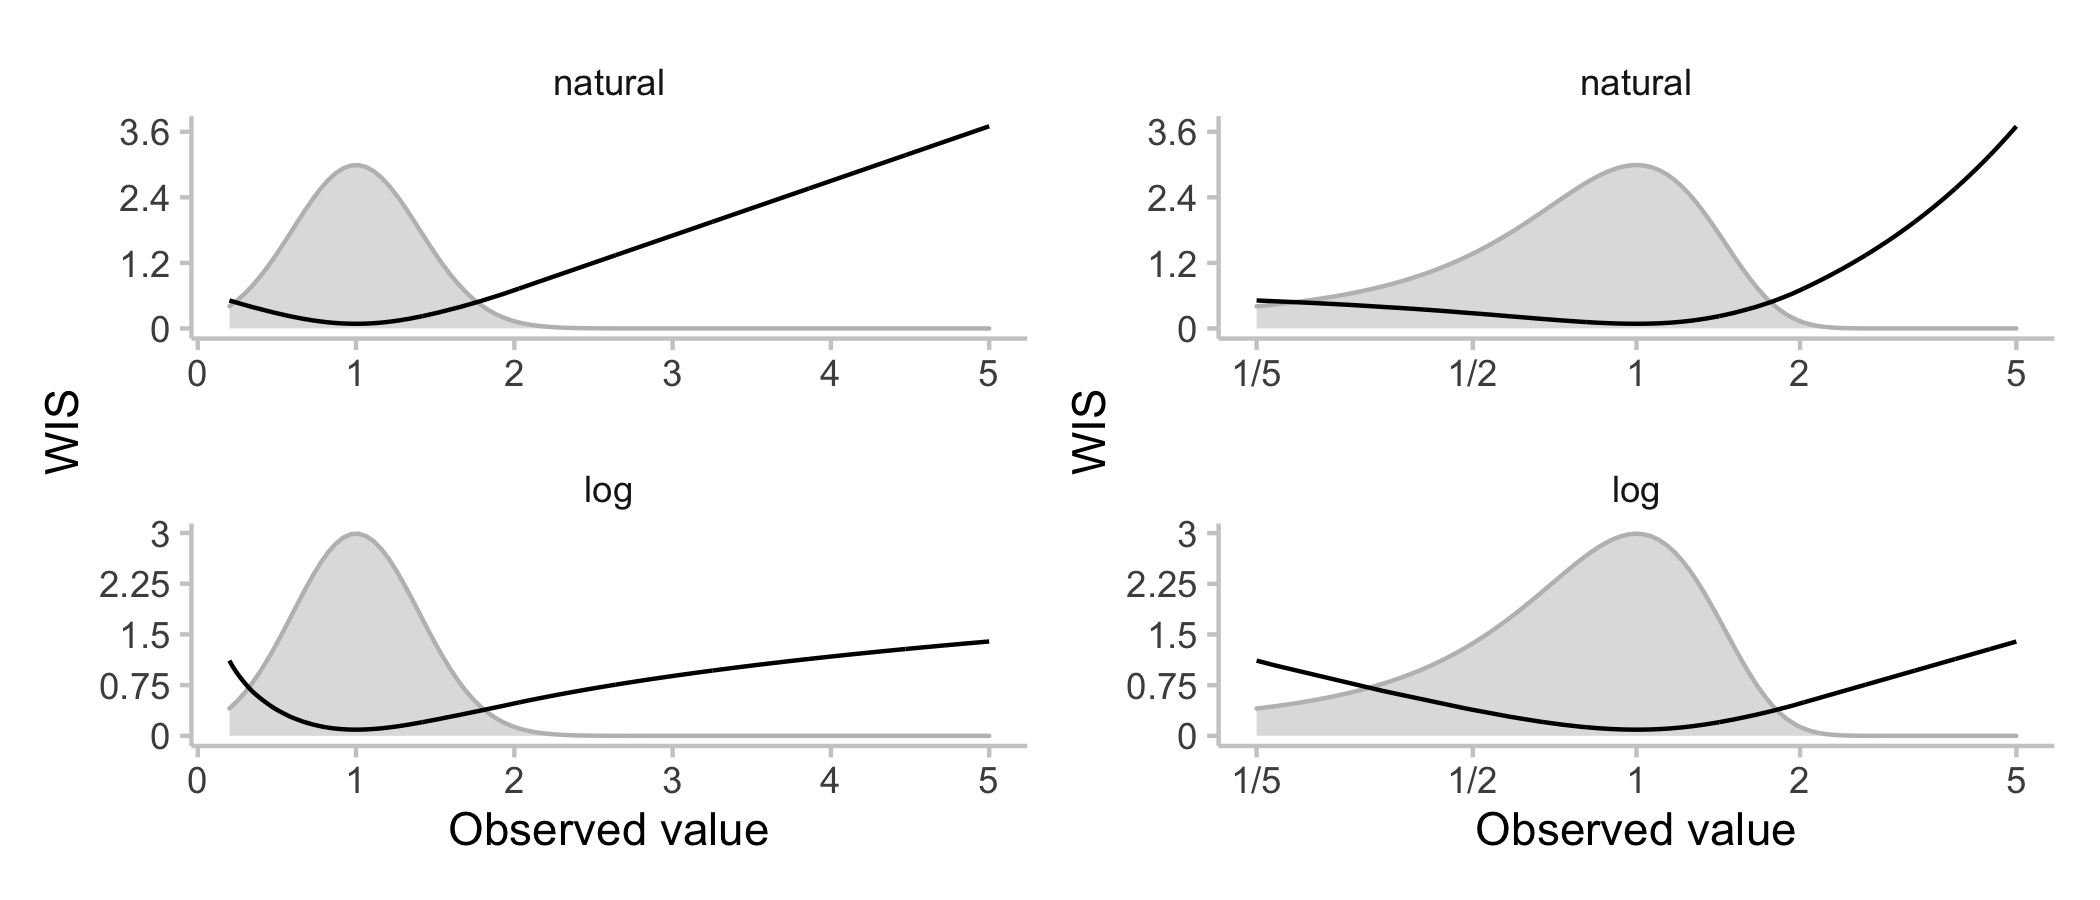
\includegraphics[width=0.99\textwidth]{output/figures/SIM-effect-log-score.png}
    \caption{Illustration of the weighted interval score (black line) for a $\mathcal{N}(1, 0.2)$ predictive distribution (density represented by the grey area) as a function of the observed value. A: Score on the natural scale, linear x-axis. B: Score on the natural scale, logarithmic x-axis. C: Score on the log scale, linear x-axis. D: Score on the log scale, logarithmic x-axis.} 
    \label{fig:change-in-scores}
\end{figure}





\subsection{Interpretation as an approximate score of the growth rate}

Computing a score based on the logarithm of the forecast and the observation is also approximately equivalent to scoring a forecast of a multiplicative growth rate of the forecast target. The growth rate is defined as
%
\begin{equation}
    g_{t, t+1} = \frac{y_{t+1} - y_t}{y_t},
\end{equation}
%
where $y_{t+1}$ is the forecast target (e.g. reported cases of COVID-19) in the future, $y_t$ is the last known observation and $g_{t, t+1}$ is the growth rate between now ($t$) and $t+1$. 
Using the growth rate, we can express the value of the forecast target in the future as such: 
%
\begin{equation}
y_{t+1} = (1 + g_{t, t+1}) \cdot y_t.
\end{equation}
%

Now consider a forecast on $\log y_{t+1}$, where again, the score is determined by the size of $\varepsilon^*_{t+1}$. Using the fact that for small values of $x$, $\log (1+ x) \approx x$, we can see that scoring forecasts on the log scale is approximately equal to scoring an additive error on the growth rate (on the natural scale), as long as the growth rate is small.
%
\begin{align}
\log y_{t+1}        &= \log \hat{y}_{t+1} + \varepsilon^*_{t+1} \\
                    &= \log ((1 + \hat{g}_{t+1}) \cdot y_{t}) + \varepsilon^*_{t+1} \\
                    &= \log (1 + \hat{g}_{t, t+1}) + \log y_t + \varepsilon^*_{t+1} \Leftrightarrow \\
\\
\varepsilon^*_{t+1}  &= \log y_{t+1} -  \log y_t - \log (1 + \hat{g}_{t, t+1}) \\    
                    &= \log (\frac{y_{t+1}}{y_t}) - \log (1 + \hat{g}_{t, t+1}) \\    
                    &= \log (1 + g_{t, t+1}) - \log (1 + \hat{g}_{t, t+1}) \\   
                    &\approx g_{t, t+1} - \hat{g}_{t, t+1} \quad \text{for small differences between } \hat{g}_{t, t+1} \text{ and } g_{t, t+1}. 
\end{align}

The score is determined by the size of $\varepsilon^*_{t+1}$, which is approximately equal to the difference between the observed and the predicted growth rate. Note that this approximation becomes increasingly inaccurate when the difference between the predicted and the actual growth rate grows (although forecasts can still be interpreted in terms of relative errors as shown above). %If this is of great concern one may want to use a different transformation such as dividing forecasts and observations by the last known values in order to score the growth rate explicitly (although this lacks the elegance of having one single transformation per time point). 

% Conveniently, the decomposition of the WIS into dispersion, overprediction and underprediction is preserved. The interpretation of the components has now changed in that they now (approximately) represent uncertainty, over-prediction, and under-prediction with the growth rate and so are independent of current incidence. 

\subsection{Effects on model rankings}
Rankings between different forecasters may change through the log transformation both when looking at aggregate scores as well as when looking at a single forecast. As an example for the effect on a single forecast, consider two forecasters, A and B. Both issue a single 50\%-prediction interval for a target which later resolves as 1. Forecaster A issues the interval [0.5, 2], while forecaster B issues [0.9. 2.5]. On the natural scale, the score would equal the dispersion of the forecast, i.e. the length of this interval (since the observed value falls within the prediction interval). Forecaster A would receive a score of $2 - 0.5$ = 1.5, beating forecaster B who would receive a score of $2.5 - 0.9 = 1.6$. When we transform the forecast, forecaster A receives a score of $\log (\frac{2}{0.5}) = 1.39$, while forecaster B obtains a score of $\log (\frac{2.6}{0.9}) = 1.06$ and now wins over forecaster A. The main difference between forecaster A and B is that forecaster A has issued a prediction interval ([0.5, 2]) that was more symmetric around the true value than the interval issued by forecaster B ([0.9. 2.6], which was more skewed). This means that in relative terms, Forecaster B was noticeably closer to the true value with the lower bound of her prediction interval, while only being slightly further away with the upper interval. This implies that scores on the log scale may treat (one-sided) outlier forecasts more leniently. 

% PARAGRAPH NEEDS SOME WORK
Overall model rankings usually differ even more when scores are averaged across multiple forecasts. The change in rankings of aggregate scores is not mainly driven by the kinds of changes in model rankings for single forecasts just discussed. Rather, as observations from exponential processes are likely to be on very different absolute scales, large observations will account for the majority of absolute score but will not dominate relative scores in the same way. When aggregating scores across metrics with different scales, for example reported cases, and hospitalisations, even an ideal (i.e. perfect) forecaster will make much larger errors when predicting case numbers than when predicting hospitalisations. Evaluating forecasts based on relative errors may help with comparing performance across different targets. However, log transforming forecasts and observations may also result in the opposite extreme, since small absolute errors (e.g. predicting 9, rather than 3 deaths) may be large in relative terms if the quantity to forecast is very small. This is especially true when forecasts are restricted to discrete values. 

\begin{figure}[h!]
    \centering
    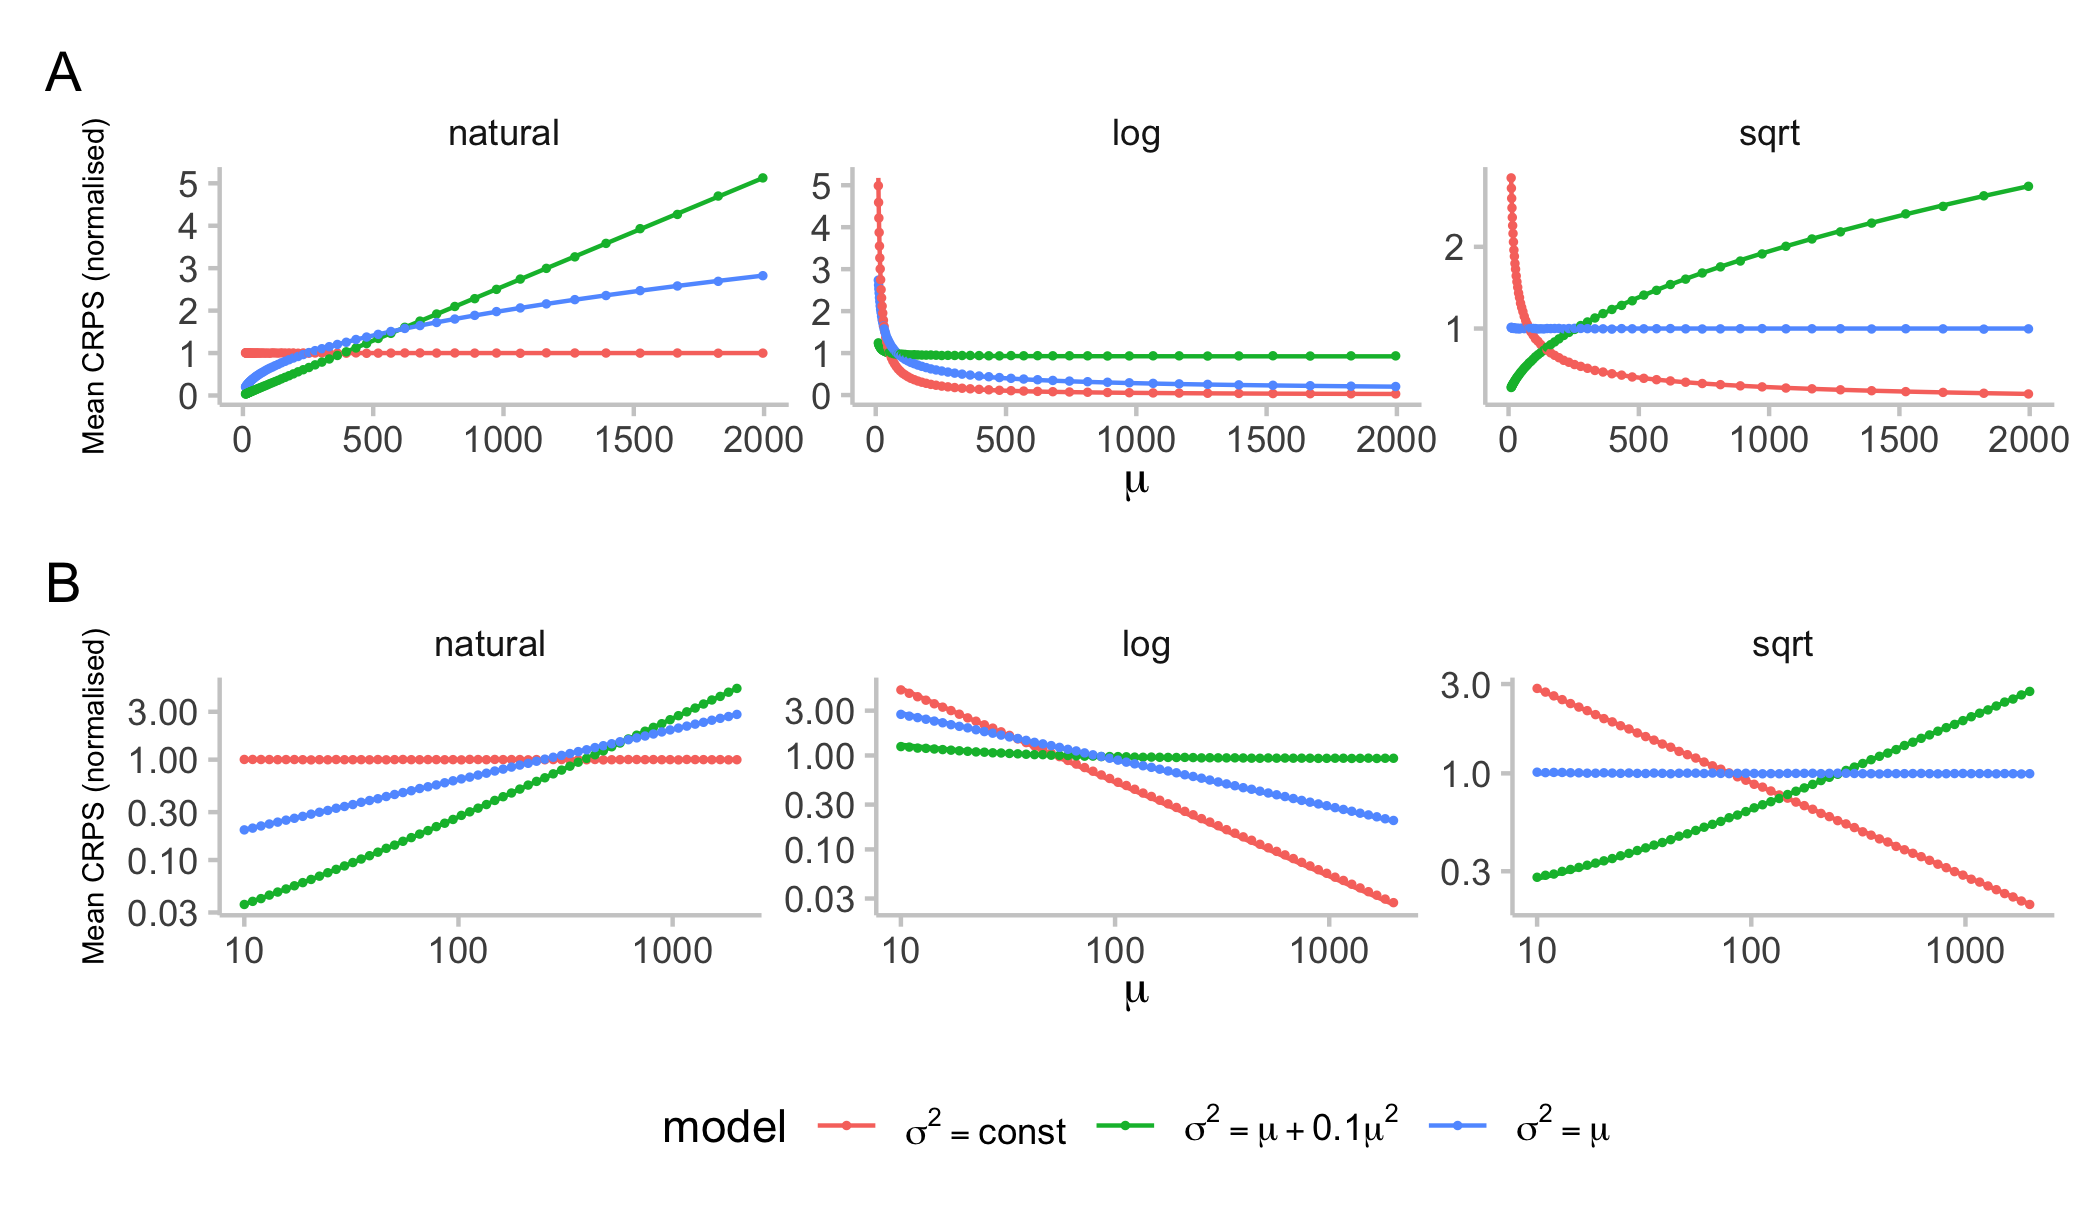
\includegraphics[width=0.99\textwidth]{output/figures/SIM-mean-state-size.png}
    \caption{Simulation showing how the relationship between mean and variance of the forecast quantity affects scores. 1,000 samples were drawn from different negative binomial distributions and scores were computed assuming an ideal forecaster (forecast distribution equal to data-generating distribution). Observations were simulated for different means of the negative-binomial distributions (representing, for example, the number of cases in differently sized states) as well as different relationships between mean and variance (representing, for example, three different infectious processes). The variance of the negative binomial is given as $\sigma^2 = \mu + \mu^2 / \theta$, meaning that for large theta the negative binomial distribution is equal to the Poisson distribution. We used values of $\theta = 0.1$ (red), 1 (green) and 1b (blue). To make the scores for the different distributions comparable, scores were normalised to one, meaning that the mean score for every distribution (red, green, blue) is one. 
    A: Normalised WIS for ideal forecasts with increasing means of three distribution with different relationships between mean and variance. B: A but with log scale axis.}
    \label{fig:SIM-wis-state-size-mean}
\end{figure}

Whether or not forecast targets with smaller quantities receive higher scores than those for targets with larger quantities, depends on the exact relationship between the mean and the variance of the quantity of interest. For simulated count data following a negative binomial distribution, for example, log predictions for small quantities receive on average higher scores than forecasts for large quantities if the mean and the variance grow at the same rate $\sigma^2 = \mu$, about equal scores when the variance grows at a rate of $\sigma^2 = \mu + \mu^2$ (Figure \ref{fig:SIM-wis-state-size-mean}), and smaller scores when the variance grows faster than that. 
% To illustrate this with count data we sampled forecasts from different negative binomial distributions. The negative binomial distribution has mean $\mu$ and variance $\sigma^2 = \mu + \mu ^2 / \theta$ and for $\lim_{\theta \to \infty}$ converges to the Poisson distribution. For large values of $\theta$, resulting in a variance approximately equal to the mean, forecasts for lower quantities on average received higher scores on the log scale (see Figure \ref{fig:SIM-wis-state-size-mean}. For $\theta = 1$ (and correspondingly, $\sigma^2 = \mu + \mu^2$, we found that scores on the log scale remained approximately constant regardless of the size of the quantity to forecast. For $\theta = 0.1$ (and $\sigma^2 = \mu + 10 \cdot \mu^2$), scores on the log scale increased with the quantity to forecast. When scored on the natural scale, a higher quantity to forecast always lead to higher scores regardless of the chosen distribution (as long as the variance grows together with the mean). 

\subsection{Practical considerations}

The log transformation is permissible (in the sense that it preserves propriety of the score), because it is a strictly monotonic transformation. Even though actual rankings between models may change, a forecaster will in expectation still minimise her score if she reports a predictive distribution that is equal to the data-generating distribution. The order of the operations matters, and applying the log transformation after scores have been computed, i.e. computing $\log S(F, y)$ results in an improper score. This is because taking the logarithm of the WIS / CRPS results in a score that does not penalise outliers enough and therefore incentivises overconfident predictions. We illustrate this point using simulated data in Figure \ref{fig:log-improper}, where it can easily be seen that overconfident models perform best in terms of the log WIS. 

\begin{figure}[h!]
    \centering
    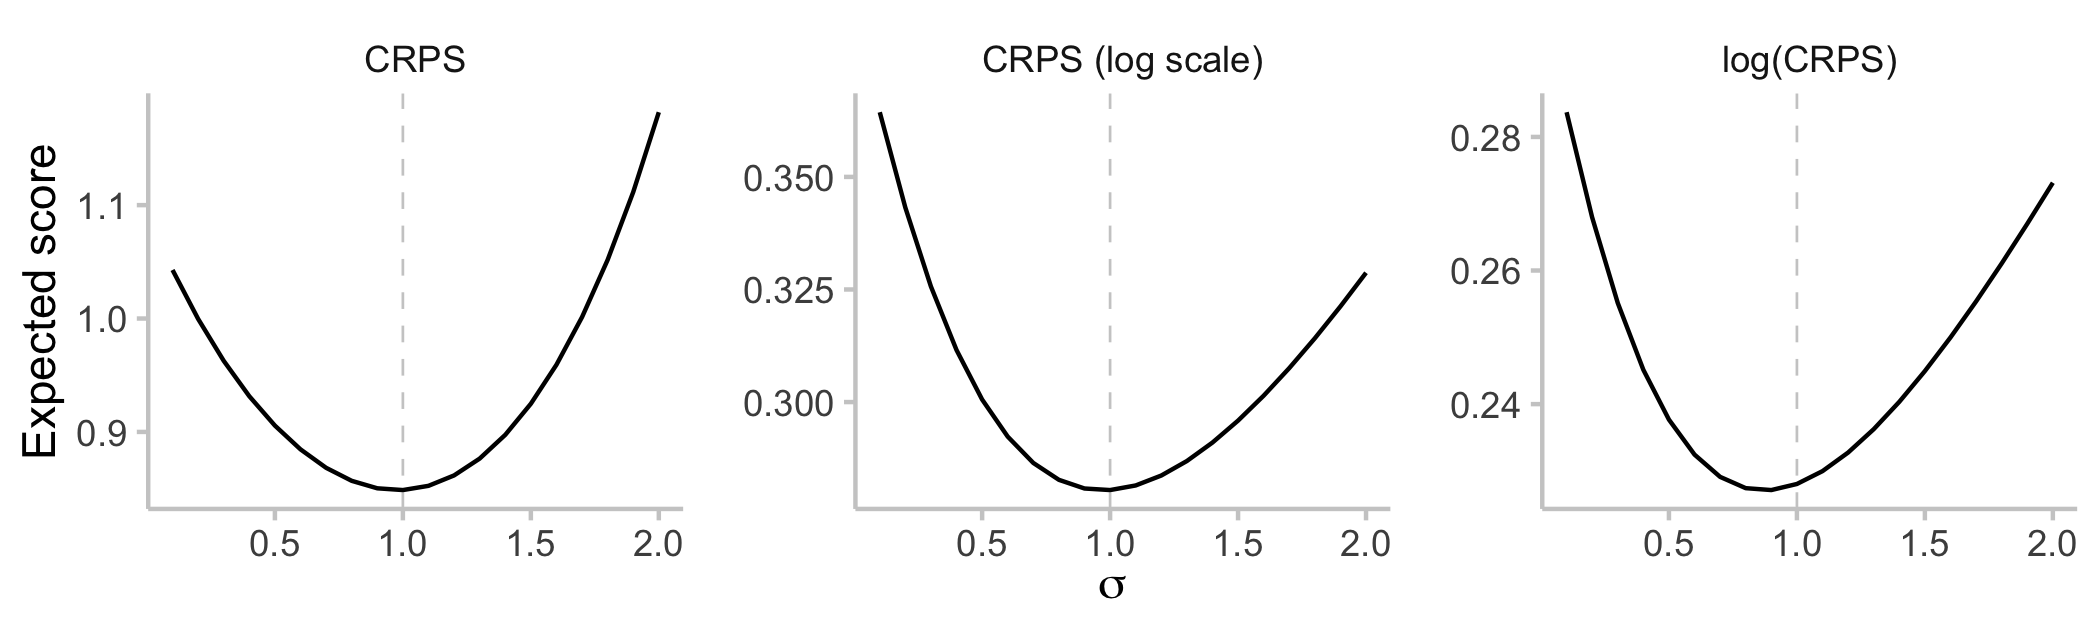
\includegraphics[width=0.99\textwidth]{output/figures/example-log-first.png}
    \caption{Scores for different forecasts evaluated the WIS and the log WIS. We simulated 1000 observations $Y_i = {\rm e}^{x_i}$, with $x_i \text{iid} \sim \mathcal{N}(0, 1)$. We then simulated 20 forecasters who would issue a predictive distribution $F = {\rm e}^{x_i}$, with $x \sim \mathcal{N}(0, \sigma)$, with values of $\sigma$ ranging from 0.1 to 2.}
    \label{fig:log-improper}
\end{figure}

In practice, one issue with the log transformation is that it cannot readily be applied to negative numbers or zero values. In addition, it may difficult to reliably evaluate relative errors when dealing with small discrete values. In an epidemiological setting that involves count data, negative values should likely be omitted entirely. One solution to deal with zeroes and small values is to also exclude those from ongoing analysis. An alternative is to add a small quantity, such as 1, to all observations and predictions before taking the logarithm as is common practice when log transforming counts. This represents a strictly monotonic transformation and therefore preserves propriety of the resulting score. The choice of the number to add influences scores and rankings, as measures of relative errors shrink when adding a constant to the forecast and the observation. Adding something to the forecasts and observations changes scores for forecasts of small quantities most, as relative errors shrink more the smaller the original value before adding a constant. In principle, it would also be possible to exploit the difference in how scores are affected in order to equalise scores for forecasts of quantities across different scales by adding a larger number (e.g. 100 or 10,000) if average scores are dominated too strongly by forecasts for small quantities. 



\section{Empirical example: the European Forecast Hub}

As an empirical example for evaluating forecasts on the natural and on the log scale we use forecasts from the European Forecast Hub \citep{europeancovid-19forecasthubEuropeanCovid19Forecast2021, sherrattPredictivePerformanceMultimodel2022}. 
The European COVID-19 Forecast Hub is one of several COVID-19 Forecast hubs (together with a Hub in the US \citep{cramerEvaluationIndividualEnsemble2021} and one in Germany and Poland \citep{bracherShorttermForecastingCOVID192021} that systematically collects, aggregated and evaluated forecasts of several COVID-19 targets created by different teams every week. Forecasts are made one to four weeks ahead into the future and follow a quantile-based format with a set of 22 quantiles plus the median ($0.01, 0.025, 0.05, ..., 0.5, ... 0.95, 0.975, 0.99$). 

The forecasts used for the purpose of this illustrations are two-week-ahead forecasts submitted between February 8 2021 and October 18 2021 for reported cases and deaths from COVID-19. We filtered all forecasts submitted to the Hub to only include models which have submitted forecasts for both deaths and cases for 4 horizons in 32 locations on at least 16 forecast dates. Where not otherwise stated, we report results for a two-week-ahead forecast horizon. 

In addition to the WIS we use pairwise comparisons \citep{cramerEvaluationIndividualEnsemble2021} to evaluate models against each other. In a first step, score ratios are computed for all pairs of models by taking the set of overlapping forecasts between the two models and dividing the score of one model over the score achieved by the other model. The relative skill for a given model is then obtained by taking the geometric mean of all score ratios which involve that model. Low values are better, and the average model receives a relative skill score of 1. 

% SECTION STRUCUTRE / IMPORTANT THINGS
% \begin{itemize}
% \item X variation gets smaller / more even
% \item X relationship with country size changes
% \item X inndividual rankings stay similar
% \item X relative skill scores change a lot
% \item deep dive into what happens for individual models
% \item scores increase across forecast horizons
% \end{itemize}
% 
% Maybe look at correlation between bias and score?
% Correlation between relative WIS contributions on the log vs. the natural scale.?

\begin{figure}[h!]
    \centering
    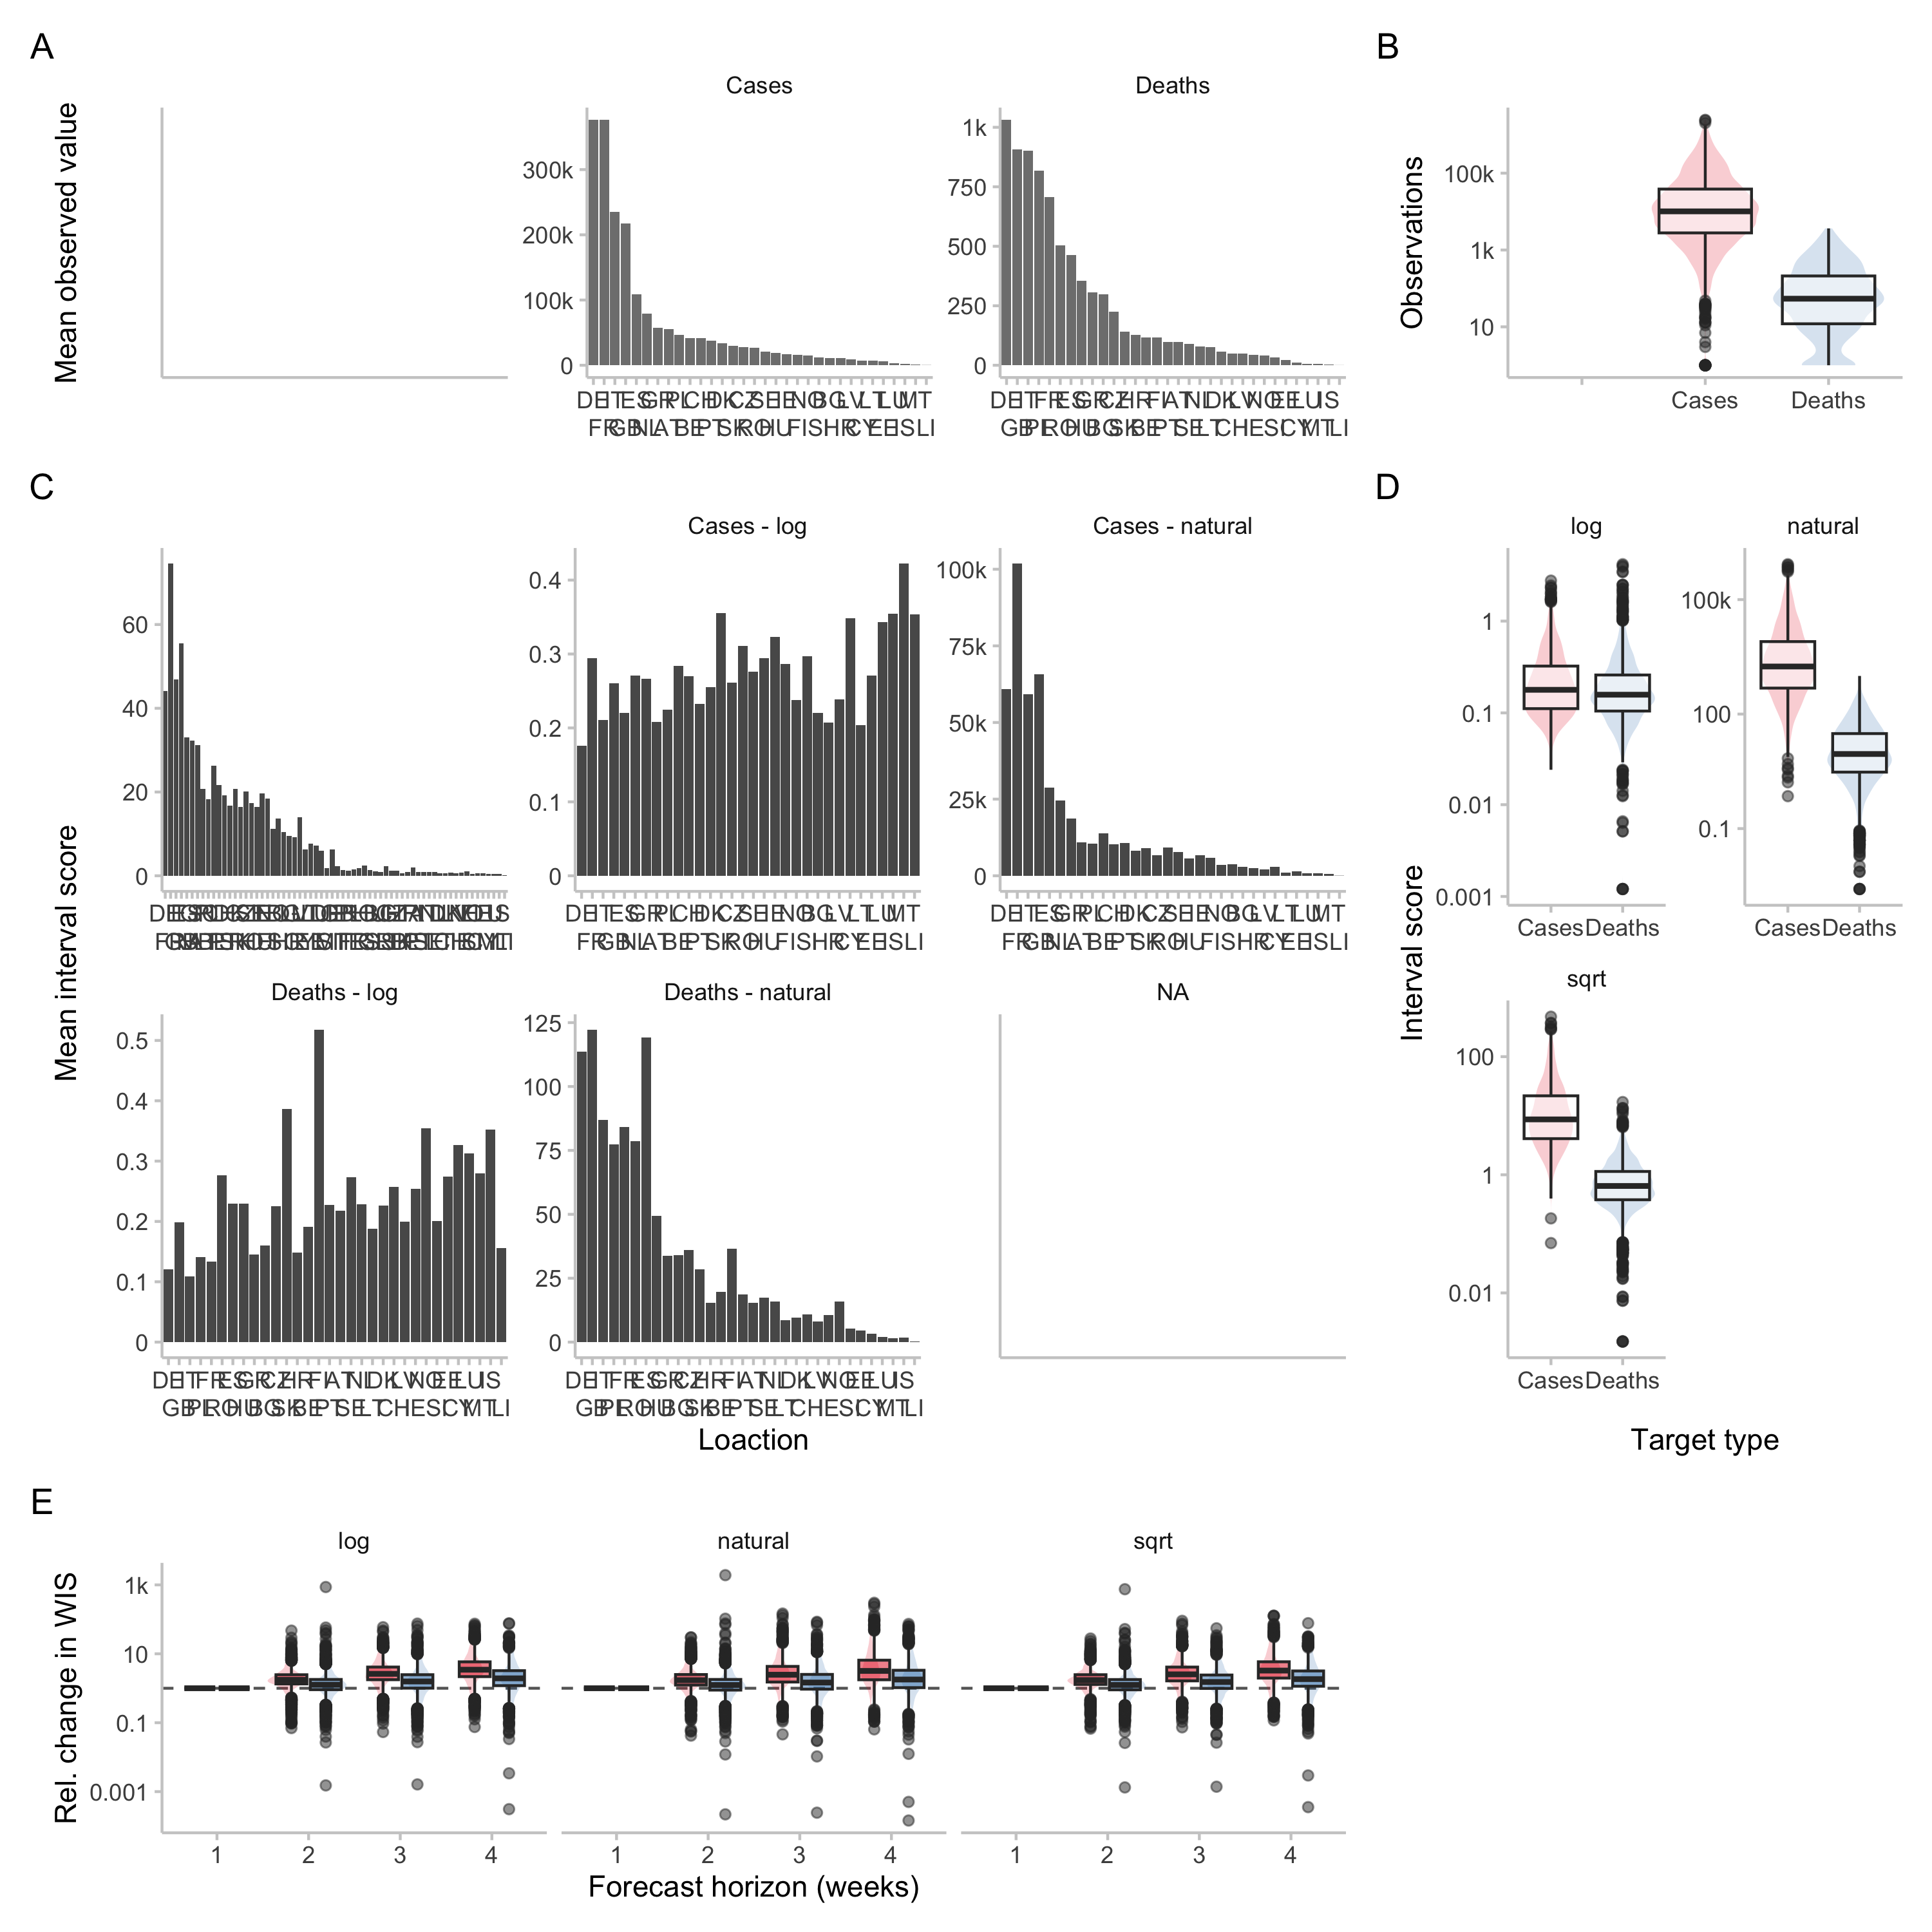
\includegraphics[width=0.99\textwidth]{output/figures/HUB-mean-obs-location.png}
    \caption{Observations and scores across locations and forecast horizons. A, Average (across all time points) of observed cases and deaths for different locations. B: Boxplot (y-axis on log-scale) of all cases and deaths. C: Scores for two-week-ahead forecasts from the EuroCOVIDhub-ensemble (averaged across all forecast dates) for different locations, evaluated on the natural as well as the logarithmic scale. D: Corresponding box-plots of all individual scores for two-week-ahead predictions. E: Boxplots for the relative change of scores for the EuroCOVIDhub-ensemble across forecast horizons. For any given forecast date and location, forecasts were made for four different forecast horizons, resulting in four scores. All scores were divided by the score for forecast horizon one.}
    \label{fig:HUB-mean-locations}
\end{figure}

Across the dataset, the average number of observed cases and deaths varied considerably by location and target type (see Figure \ref{fig:HUB-mean-locations}A and B). On the natural scale, scores also varied considerably across targets (see Fig \ref{fig:HUB-mean-locations}D) and locations (see Fig \ref{fig:HUB-mean-locations}C). On the log scale, scores were more evenly distributed between targets (see Fig \ref{fig:HUB-mean-locations}D) and locations (see Fig \ref{fig:HUB-mean-locations}). Both on the natural scale as well as on the log scale, scores increased considerably with increasing forecast horizon (see Figure \ref{fig:HUB-mean-locations}E). The increase was more pronounced for cases than for deaths. We hypothesise that this increase in scores across horizons represents the relative difficulty to forecast values into the future, which was noticeable both on the natural as well as the logarithmic scale. 

\begin{figure}[h!]
    \centering
    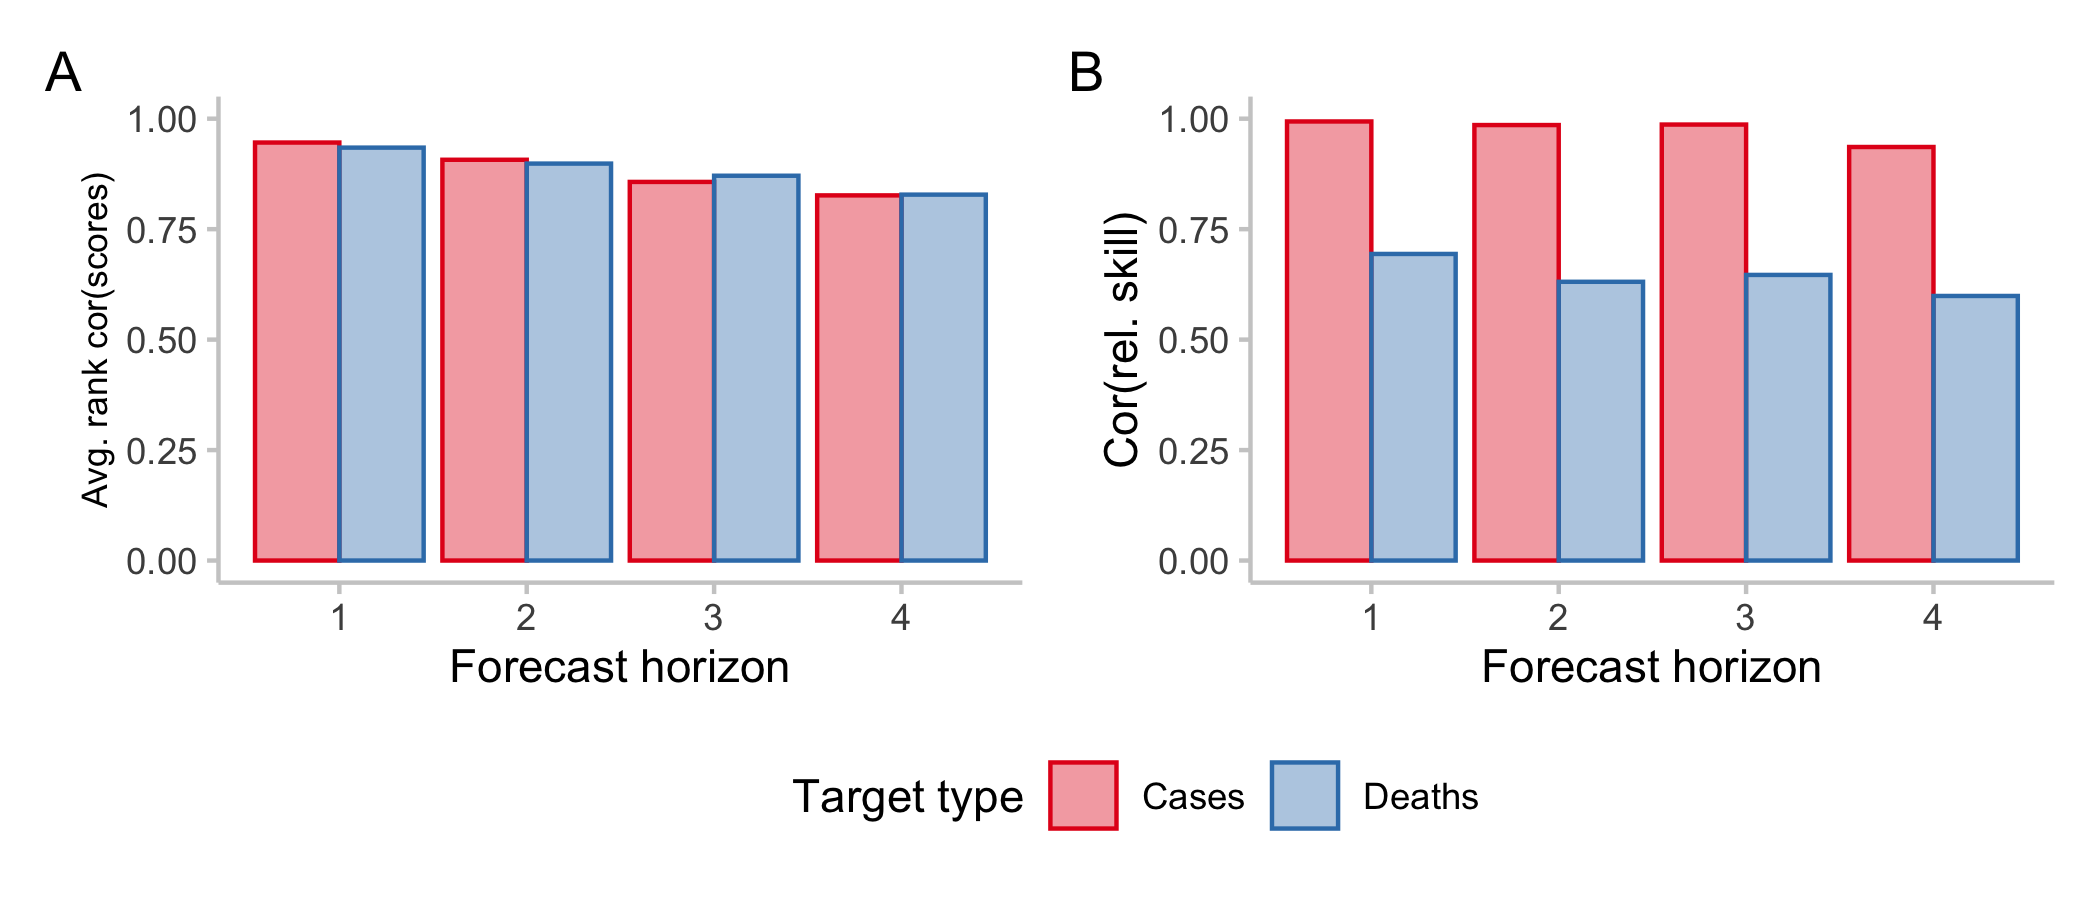
\includegraphics[width=0.99\textwidth]{output/figures/HUB-correlations.png}
    \caption{Correlations between observations and scores. A: Mean WIS for two-week-ahead predictions of the EuroCOVIDhub-ensemble against the average number of observations in a location. B: Average Spearman CHECK AGAIN (rank-) correlation of scores for individual forecasts from \textit{all} models. For every individual target (defined by a combination of forecast date, target type, horizon, location), one score was obtained per model. Then, the rank correlation was computed between the scores for all models on the natural scale vs. on the log scale. All rank correlations were averaged and stratified by horizon and target type. C: Correlation between relative skill scores. For every forecast horizon and target type, a separate rel. skill score was computed per model using pairwise comparisons. The plot shows the correlation between the rel. skill scores on the natural vs. on the log scale.}
    \label{fig:HUB-cors}
\end{figure}

As expected on the natural scale, scores correlate strongly with the average number of observed cases and deaths (Spearman correlation: XX and XX) in a given country (see Fig \ref{fig:HUB-mean-locations}A, B).
This relationship is not evident on the log scale, where correlation is much weaker and maybe slightly negative (Spearman correlation: XX and XX), implying larger scores for for countries with lower mean incidences. 


\begin{figure}[h!]
    \centering
    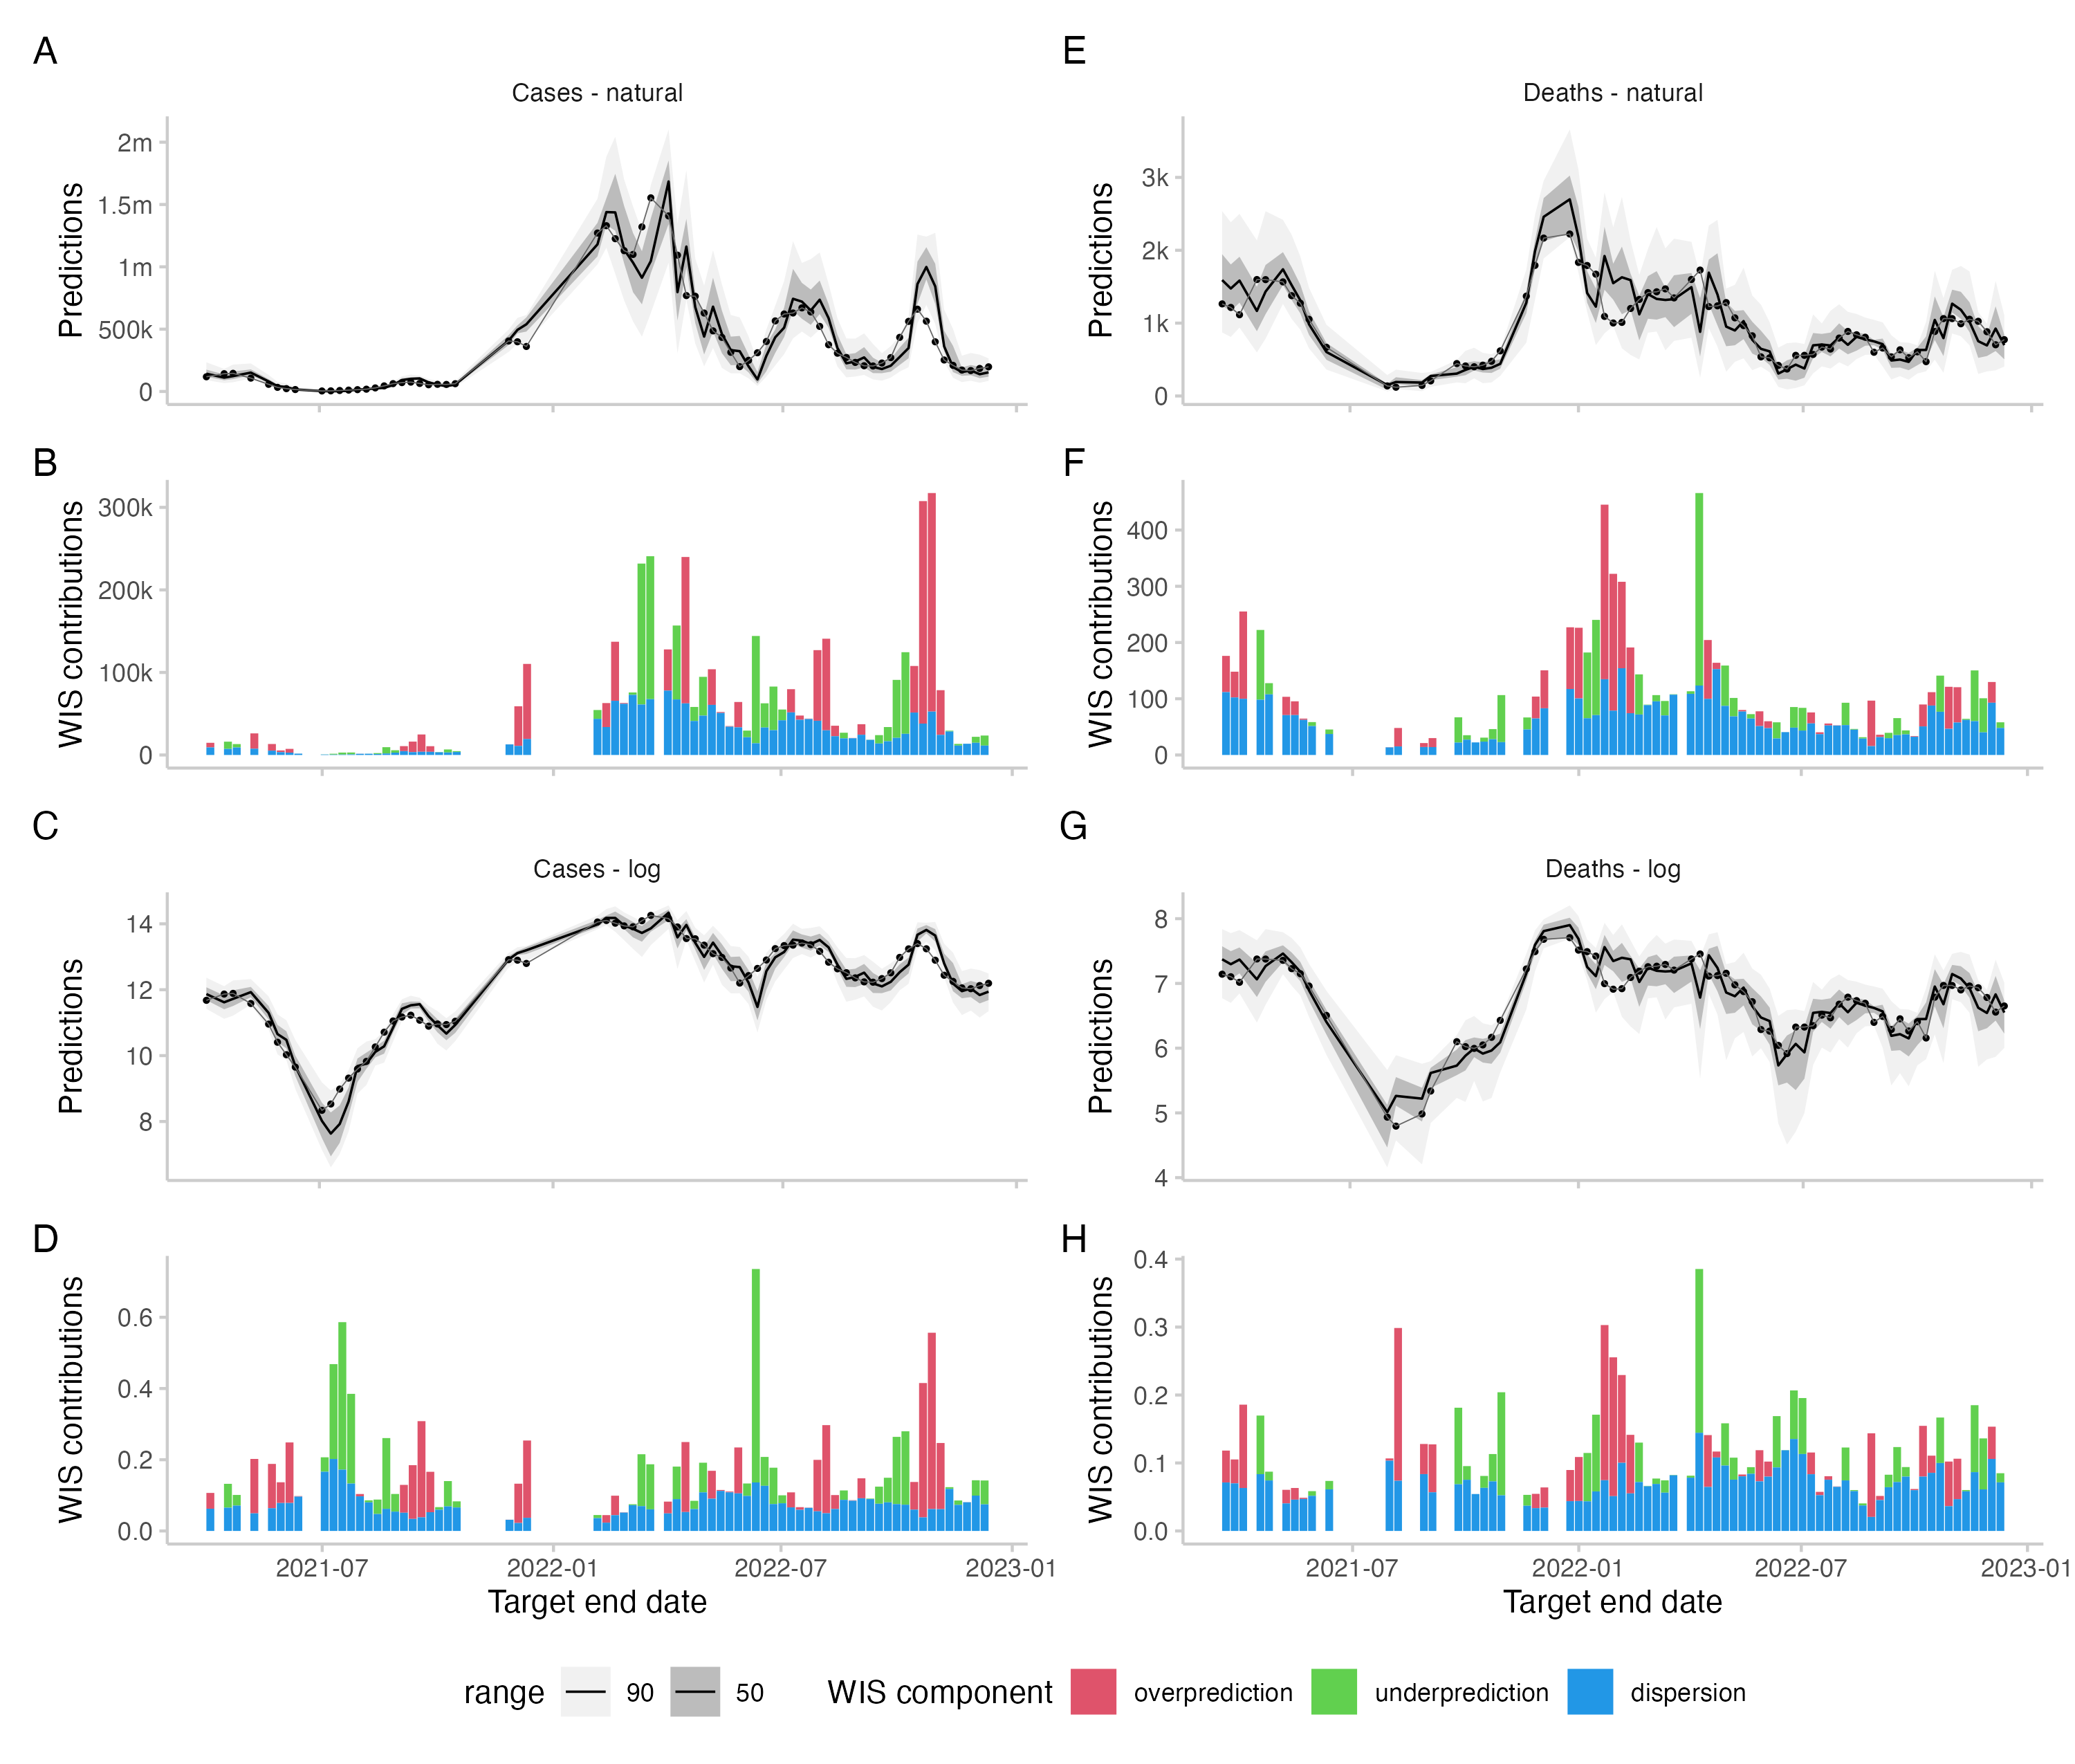
\includegraphics[width=0.99\textwidth]{output/figures/HUB-model-comparison-ensemble.png}
    \caption{
    Forecasts and scores for two-week-ahead predictions from the EuroCOVIDhub-ensemble made in Germany. A, E: 50\% and 90\% prediction intervals and observed values for cases and deaths on the natural scale. B, F: Corresponding scores. C, G: Forecasts and observations on the log scale. D, H: Corresponding scores. 
    }
    \label{fig:HUB-model-comparison-ensemble}
\end{figure}


For \textit{individual} forecasts, rankings between models for single forecasts are mostly preserved, with differences increasing across forecast horizons (see Figure \ref{fig:HUB-cors}). When evaluating performance \textit{across} different forecasts and forecast targets, relative skill scores of the models change considerably. The change is stronger for cases than for deaths (Figure \ref{fig:HUB-cors}XX) and tends to increase with increasing forecast horizon. 

When comparing examples of forecasts on the natural scale with log-transformed ones (see Figures XX, XX, XX) a few interesting patterns emerge. Missing the peak, i.e. predicting increasing numbers while actual observations are already falling, tends to contribute a lot to overall scores on the natural scale (see forecasts in May in Figure XXA, B). On the log scale, these have less of an influence, as errors are smaller in relative terms (see panels C and D). We hypothesise that the larger divergence in scores for cases (compared to scores for deaths) displayed in Figure \ref{fig:HUB-pairwise}C is related to the fact that outlier forecasts missing the peak are more common for cases than for deaths. 
Conversely, failure to predict an upswing while numbers are still low, is not severely punished on the natural scale (see forecasts in July in Figure XX A, B), as overall absolute errors are low. On the log scale, missing lower inflection points tends to lead to more severe penalties (see panels C and D). One can also observe that on the natural scale, scores tend to track the overall level of the target quantity (compare for example forecasts for March-July with forecasts for September-October in Figure XXE, F). On the log scale, scores increase whenever forecasts are far away from the truth in relative terms, regardless of the overall level of observations. 

Furthermore, including very low numbers in the confidence intervals may lead to very high scores on the log-scale. This may be an issue especially when forecasting small quantities. Figure \ref{fig:HUB-model-comparison-baseline} shows forecasts and scores for the baseline model, which had zero included in its 50 percent intervals for the forecasts in XX to XX, leading to excessive dispersion values on the log scale. Notwithstanding the general concern, one can argue that in the specific example (at least for cases) including zero in the prediction intervals was unreasonable and rightly penalised given that case numbers were in the thousands. 

\begin{figure}[h!]
    \centering
    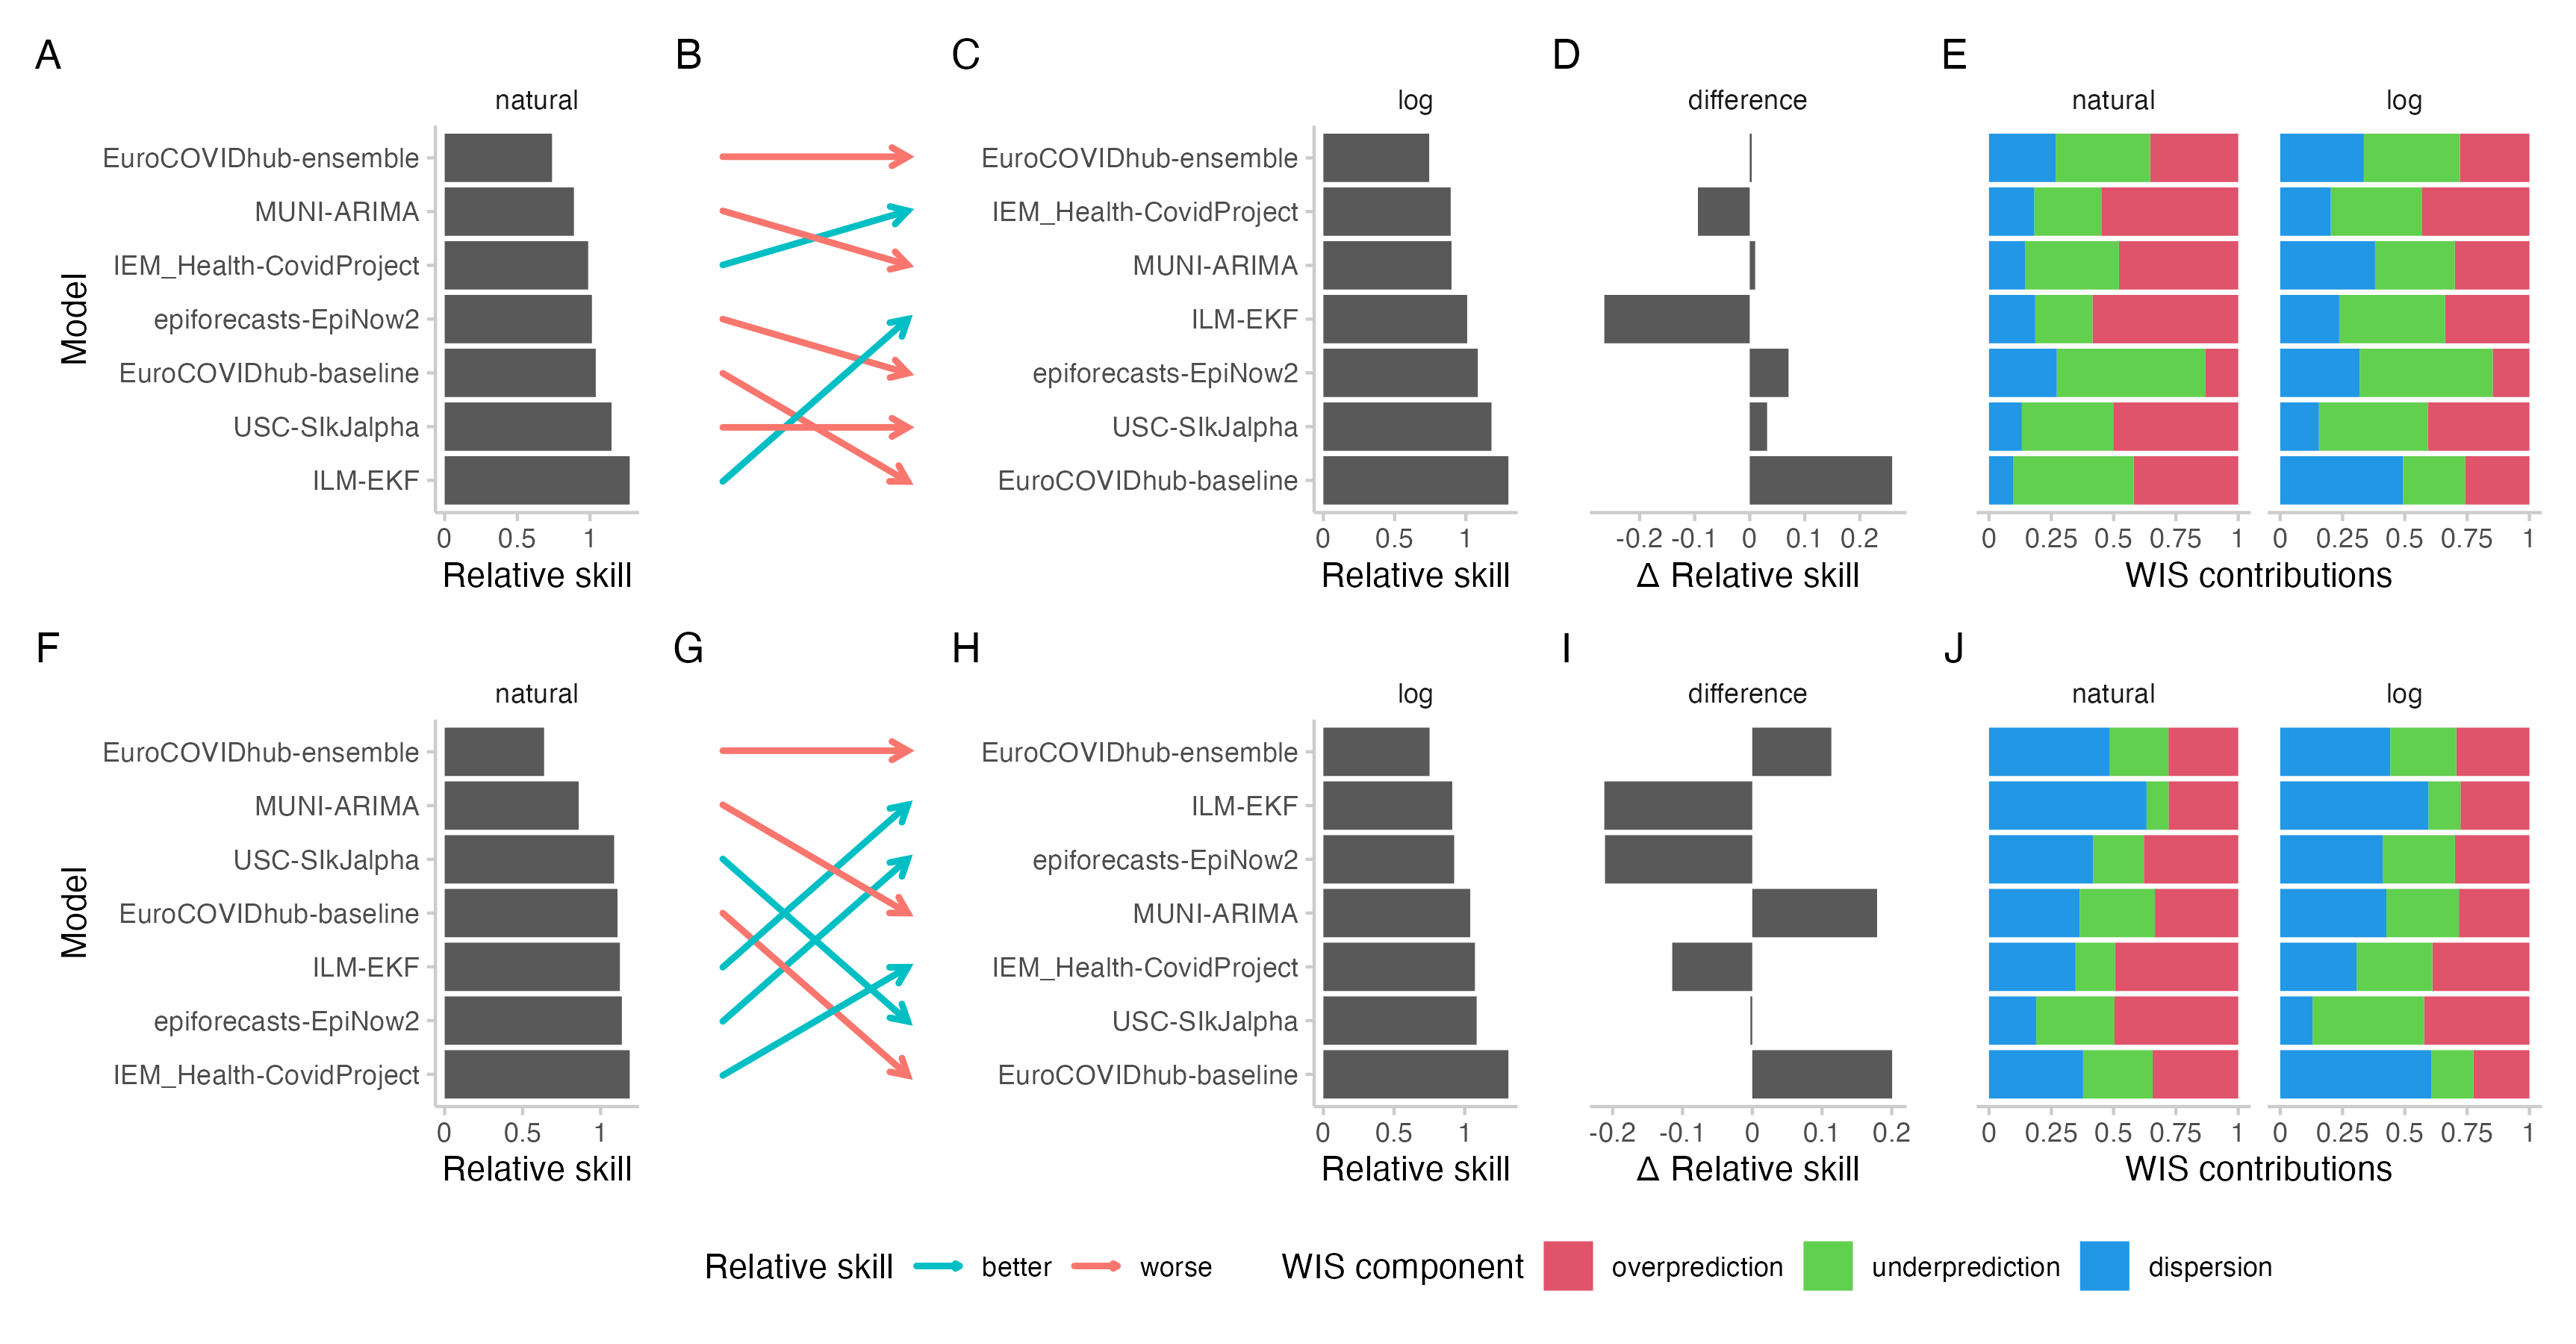
\includegraphics[width=0.99\textwidth]{output/figures/HUB-pairwise-comparisons.png}
    \caption{Changes in model ratings as measured by relative skill for two-week-ahead predictions. Top row: cases, bottom row: deaths. NEED TO CHANGE THE ANNOTATION LEVELS.}
    \label{fig:HUB-pairwise}
\end{figure}


Evaluating the rank order of forecasts from the ECDC forecast hub we saw that scoring after a log transform altered the order of forecast models. In particular, we note that models that are known to not make use of a exponential error model and to be biased towards under-prediction, such the the MUNI-ARMA model were ranked lower when using a log transform. A submission by the authors of this study, the epiforecasts-EpiNow2 forecast model, was the most impacted by the change to log scale scoring moving from last place for reported cases to 4th place. This makes sense given that it explicitly models errors on an exponential scale, and is relatively unbiased meaning it may be over-penalised due to over-prediction during periods of peak incidence. Interestingly, other models that are growth rate based, such as the LANL-GrowthRate forecaster, do less well after a log-transform. Encouragingly for the ECDC forecast Hub the Hub ensemble, which is the forecast the organisers suggest forecast consumers make use of, remains one of the top forecasts across scoring schemes and indeed ranks higher for reported cases when a log transform is used.

% Observations were overdispersed, meaning that for a given location, the variance in observations exceeds the mean of all observed values (see Figure \ref{fig:HUB-variance-mean}). 
%Could fit a model var = alpha * x2 + beta *x
%This is in line with the observation that the association between variance is smaller than mu^2 + mu, meaning that we would expect this. 



\section{Discussion}
\label{sec:discussion}

In this paper we proposed a log transformation of forecasts and observed values prior to evaluation with the WIS (or CRPS) in order to address issues that arise when evaluating epidemiological forecasts based on a measure of absolute error. We gave a mathematical intuition for the transformation and showed that scores on the log scale can be interpreted as a) a measure of relative (multiplicative) prediction errors, as well as b) as an approximate score for a forecast of the multiplicative growth rate of the target quantity. 
When applying this approach to forecasts from the European COVID-19 Forecast Hub, we found overall scores to be more equal across, time, location and target type (cases, deaths). Scores on the log scale were much less influenced by the overall incidence level in a country, and showed a slight tendency to be higher in locations with a very incidences. We found that model rankings changed noticeably, favouring models like epiforecasts-EpiNow2 which explicitly has an exponential error structure, and disfavouring models like MUNI-ARIMA which is purely statistical model with a linear error structure. On the natural scale, missing the peak and overshooting was more severely penalised, while missing the nadir and a following upswing in numbers tended to be more severely penalised on the log scale than on the natural scale. 

\paragraph{strengths and weaknesses}

Applying a log transformation prior to the WIS means that forecasts are evaluated in terms of relative errors and errors on the multiplicative growth rate, rather than absolute errors. The most important strength of this approach is that the evaluation better accommodates the exponential nature of epidemiological process and the types of errors forecasters who accurately model those processes are expected to make. The log transformation also helps avoid issues with scores being strongly influenced by the order of magnitude of the forecast quantity, which can be seen when evaluating forecasts on the natural scale. 
A potential downside is that forecast evaluation is unreliable in situations where observed values are zero or very small. Similarly, locations with lower incidences may get disproportionate weight (i.e. high scores) when evaluating forecasts on the log scale. \cite{bracherEvaluatingEpidemicForecasts2021} argue that the large weight given to forecasts for locations with high incidences is a desirable property, as it reflects performance on the targets we should care about most. On the other hand, scoring forecasts on the log scale may be less influenced by single outliers and better reflect consistent performance across time, space, and forecast targets. It also gives higher weight to another type of situation one may care about, namely one in which numbers start to rise from a previously low level. 
While scores on the log scale can always be interpreted as a measure of relative (multiplicative) predictive performance, the interpretation as a score for a forecast of the multiplicative growth rate is only approximate. If one is explicitly interested in scoring a forecast of the growth rate, it may be better to use a different transformation, e.g. dividing every forecast and corresponding observed value by the previously last observed value when the forecast was made. 

It is important to note that the log transformation is only one of many transformation that may be useful and appropriate in an epidemiological context. One easy transformation is to divide all forecasts by the population in a location, in order to obtain forecasts standardised incidences per e.g. 100,000 inhabitants. A second transformation was mentioned above, namely converting forecasts into forecasts for the multiplicative growth rate by dividing by the last observed value. One could also think about applying a Box-Cox or a square-root transformation in order to stabilise the variance of the forecasts. Another promising transformation would be to divide each forecast by the forecast of the previous week (and observations by the observation of the previous week), in order to obtain forecasts for week-to-week growth rates. This would be akin to evaluating the shape of the predicted trajectory against the shape of the observed trajectory (for a different approach to evaluation the shape of a forecast, see https://arxiv.org/abs/2209.04035). This, unfortunately is not well defined in the context of forecasts stored as predictive quantiles, as the growth rate of the $\alpha$-quantile may be different from the $\alpha$-quantile of the growth-rate, but may be an interesting approach if predictive samples are available. What makes this approach of transforming forecasts before scoring particularly interesting is the possibility to construct composite scores as a weighted sum of scores based on different transformations. This would allow forecast consumers to assign explicit weights to different qualities of the forecasts they might care about. 

Exploring these different transformations is a promising avenue for future work that could help bridge the gap between modellers and policy makers by providing scoring rules that better reflect what forecast consumers actually care about. We have showed that the log transformation can lead to significant changes in the relative rankings of models against each other, with potentially important implications for decision makers who rely on the knowledge of past performance to make a decision about which forecasts should inform future decisions. We think it would therefore be a good idea to show different versions of the WIS in order to obtain a richer picture of model performance. While we have provided a small case study, more work needs to be done to better understand the effects of applying a log transformation in different contexts and how it might affect decision making. 



 %COULD ALSO MAKE A NICE PLOT ABOUT OUTLIERS, where we look at the effect of outliers. but maybe that is already included in the plot in Figure 1. 
% could make an analysis re outliers: how do scores change if we remove the 1 or 2 worst forecasts? The one or two best forecasts?


\newpage

\appendix
\section{Supplementary information}

\begin{table}[h!]
    \centering
    
    \begin{tabular}{lllcc}
    \toprule
    target\_type & quantity & measure & natural & log\\
    \midrule
    Cases & Observations & mean & 20308 & 8.39\\
    Cases & Observations & sd & 43405 & 2.11\\
    Cases & Observations & var & 1884002308 & 4.46\\
    \addlinespace
    Deaths & Observations & mean & 259 & 3.79\\
    Deaths & Observations & sd & 532 & 2.11\\
    Deaths & Observations & var & 283492 & 4.46\\
    \addlinespace
    \hline
    \addlinespace
    Cases & WIS & mean & 4544 & 0.28\\
    Cases & WIS & sd & 17585 & 0.49\\
    \addlinespace
    Deaths & WIS & mean & 28 & 0.22\\
    Deaths & WIS & sd & 67 & 0.26\\
    \bottomrule
    \end{tabular}
    \caption{Table with summary statistics for observations and scores for forecasts from the ECDC data set.}
    \label{tab:HUB-summary}
\end{table}



\begin{figure}[h!]
    \centering
    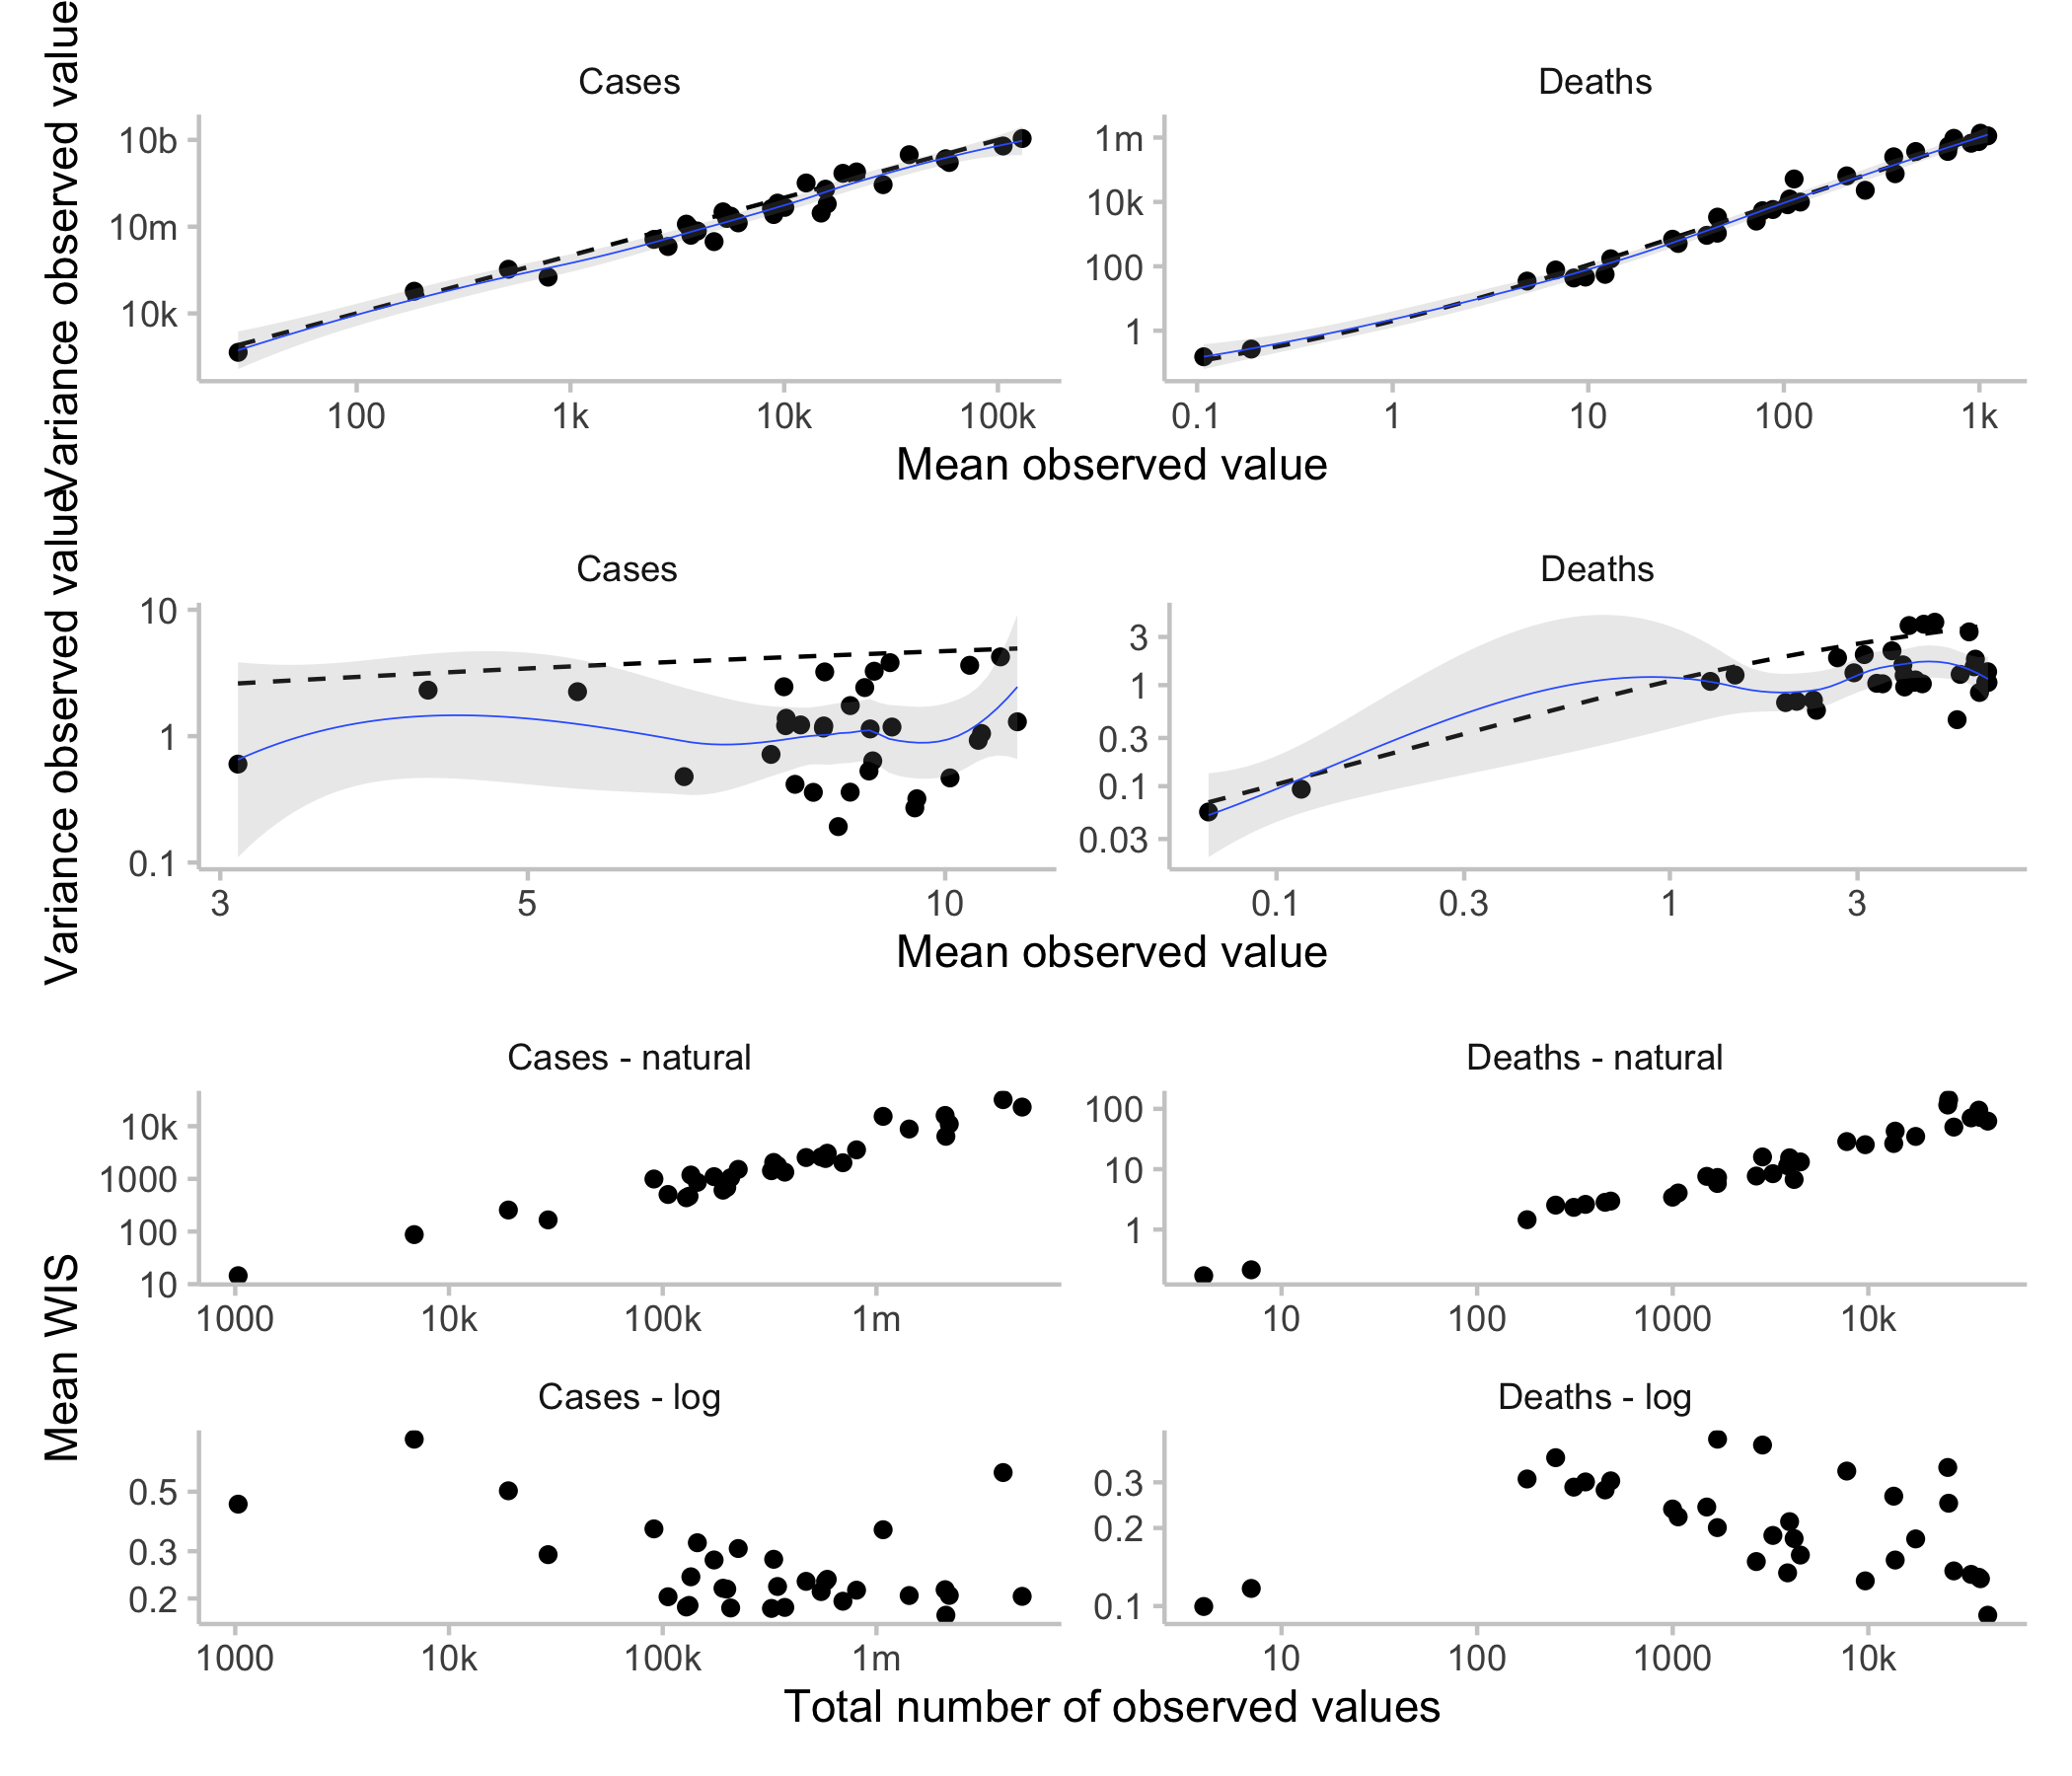
\includegraphics[width=0.99\textwidth]{output/figures/HUB-mean-scores-vs-total-log-log.png}
    \caption{My current thinking is that the top row is helpful, as it explalins what the mean / var relationship is which is relevant for how much weight small countries get. I think the 2nd row is just completely useless. The 3rd and 4th row may be helpful. In some sense it is duplicated information from above, but it gives some nice intuiton for the correlations. I could alternatively also turn it into a correlation plot and add it to the other one. }
    \label{fig:HUB-mean-scores-total-loglog}
\end{figure}


\subsection{Additional information on the WIS} \label{wis}

The Weighted Interval Score is a proper scoring rule. WIS values are always larger or equal than zero and lower values imply better performance. The WIS can be decomposed into a dispersion component and penalties for over- and under-prediction. For a single prediction interval, the interval score is computed as 
\begin{align}
 IS_\alpha(F,y) &= (u-l) + \frac{2}{\alpha} \cdot (l-y) \cdot 1(y \leq l) + \frac{2}{\alpha} \cdot (y-u) \cdot 1(y \geq u) \\
 &= \text{dispersion} + \text{underprediction} + \text{overprediction},    
\end{align}

where $1()$ is the indicator function, $y$ is the observed value, and $l$ and $u$ are the $\frac{\alpha}{2}$ and $1 - \frac{\alpha}{2}$ quantiles of the predictive distribution $F$, i.e. the lower and upper bound of a single central prediction interval. For a single forecast interval, the interval score is the width of the prediction interval, if it covers the observed value, and the absolute error between the forecast and the lower (or upper, respectively) interval boundary. For a set of $K$ prediction intervals and the median $m$, the WIS is computed as a weighted sum, 
\begin{equation}
\text{WIS} = \frac{1}{K + 0.5} \cdot \left(w_0 \cdot |y - m| + \sum_{k = 1}^{K} w_k \cdot IS_{\alpha}(F, y)\right),    
\end{equation} 
where $w_k$ is a weight for every interval. Usually, $w_k = \frac{\alpha_k}{2}$ and $w_0 = 0.5$. 


The WIS is closely related to the continuous ranked probability score (CRPS) [Cite Gneiting 2007], which itself can be understood as a generalisation of the absolute error to probabilistic forecasts. For an increasing set of equally-spaced prediction intervals the WIS converges to the CRPS and shares many of its properties. More information on the CRPS is provided in section \ref{crps} in the SI. 

\subsection{Additional information on the CRPS} \label{crps}

The CRPS measures the distance of the predictive distribution to the observed data-generating distribution as 

\begin{equation}
    \text{CRPS}(F, y) = \int_{-\infty}^\infty \left( F(x) - 1(x \geq y) \right)^2 dx,
\end{equation}

where y is the true observed value and F the CDF of predictive distribution. Often the following alternative representation is used
\begin{equation}
    \text{CRPS}(F, y) = \frac{1}{2} \mathbb{E}_{F} |X - X'| - \mathbb{E}_P |X - y|,
\end{equation}
  
where $X$ and $X'$ are independent realisations from the predictive distributions $F$ with finite first moment and $y$ is the true value. In this representation we can simply replace $X$ and $X'$ by samples sum over all possible combinations to obtain the CRPS.  




\subsection{Additional figures}

NUMBER OF AVAILABLE FORECASTS


\begin{figure}[h!]
    \centering
    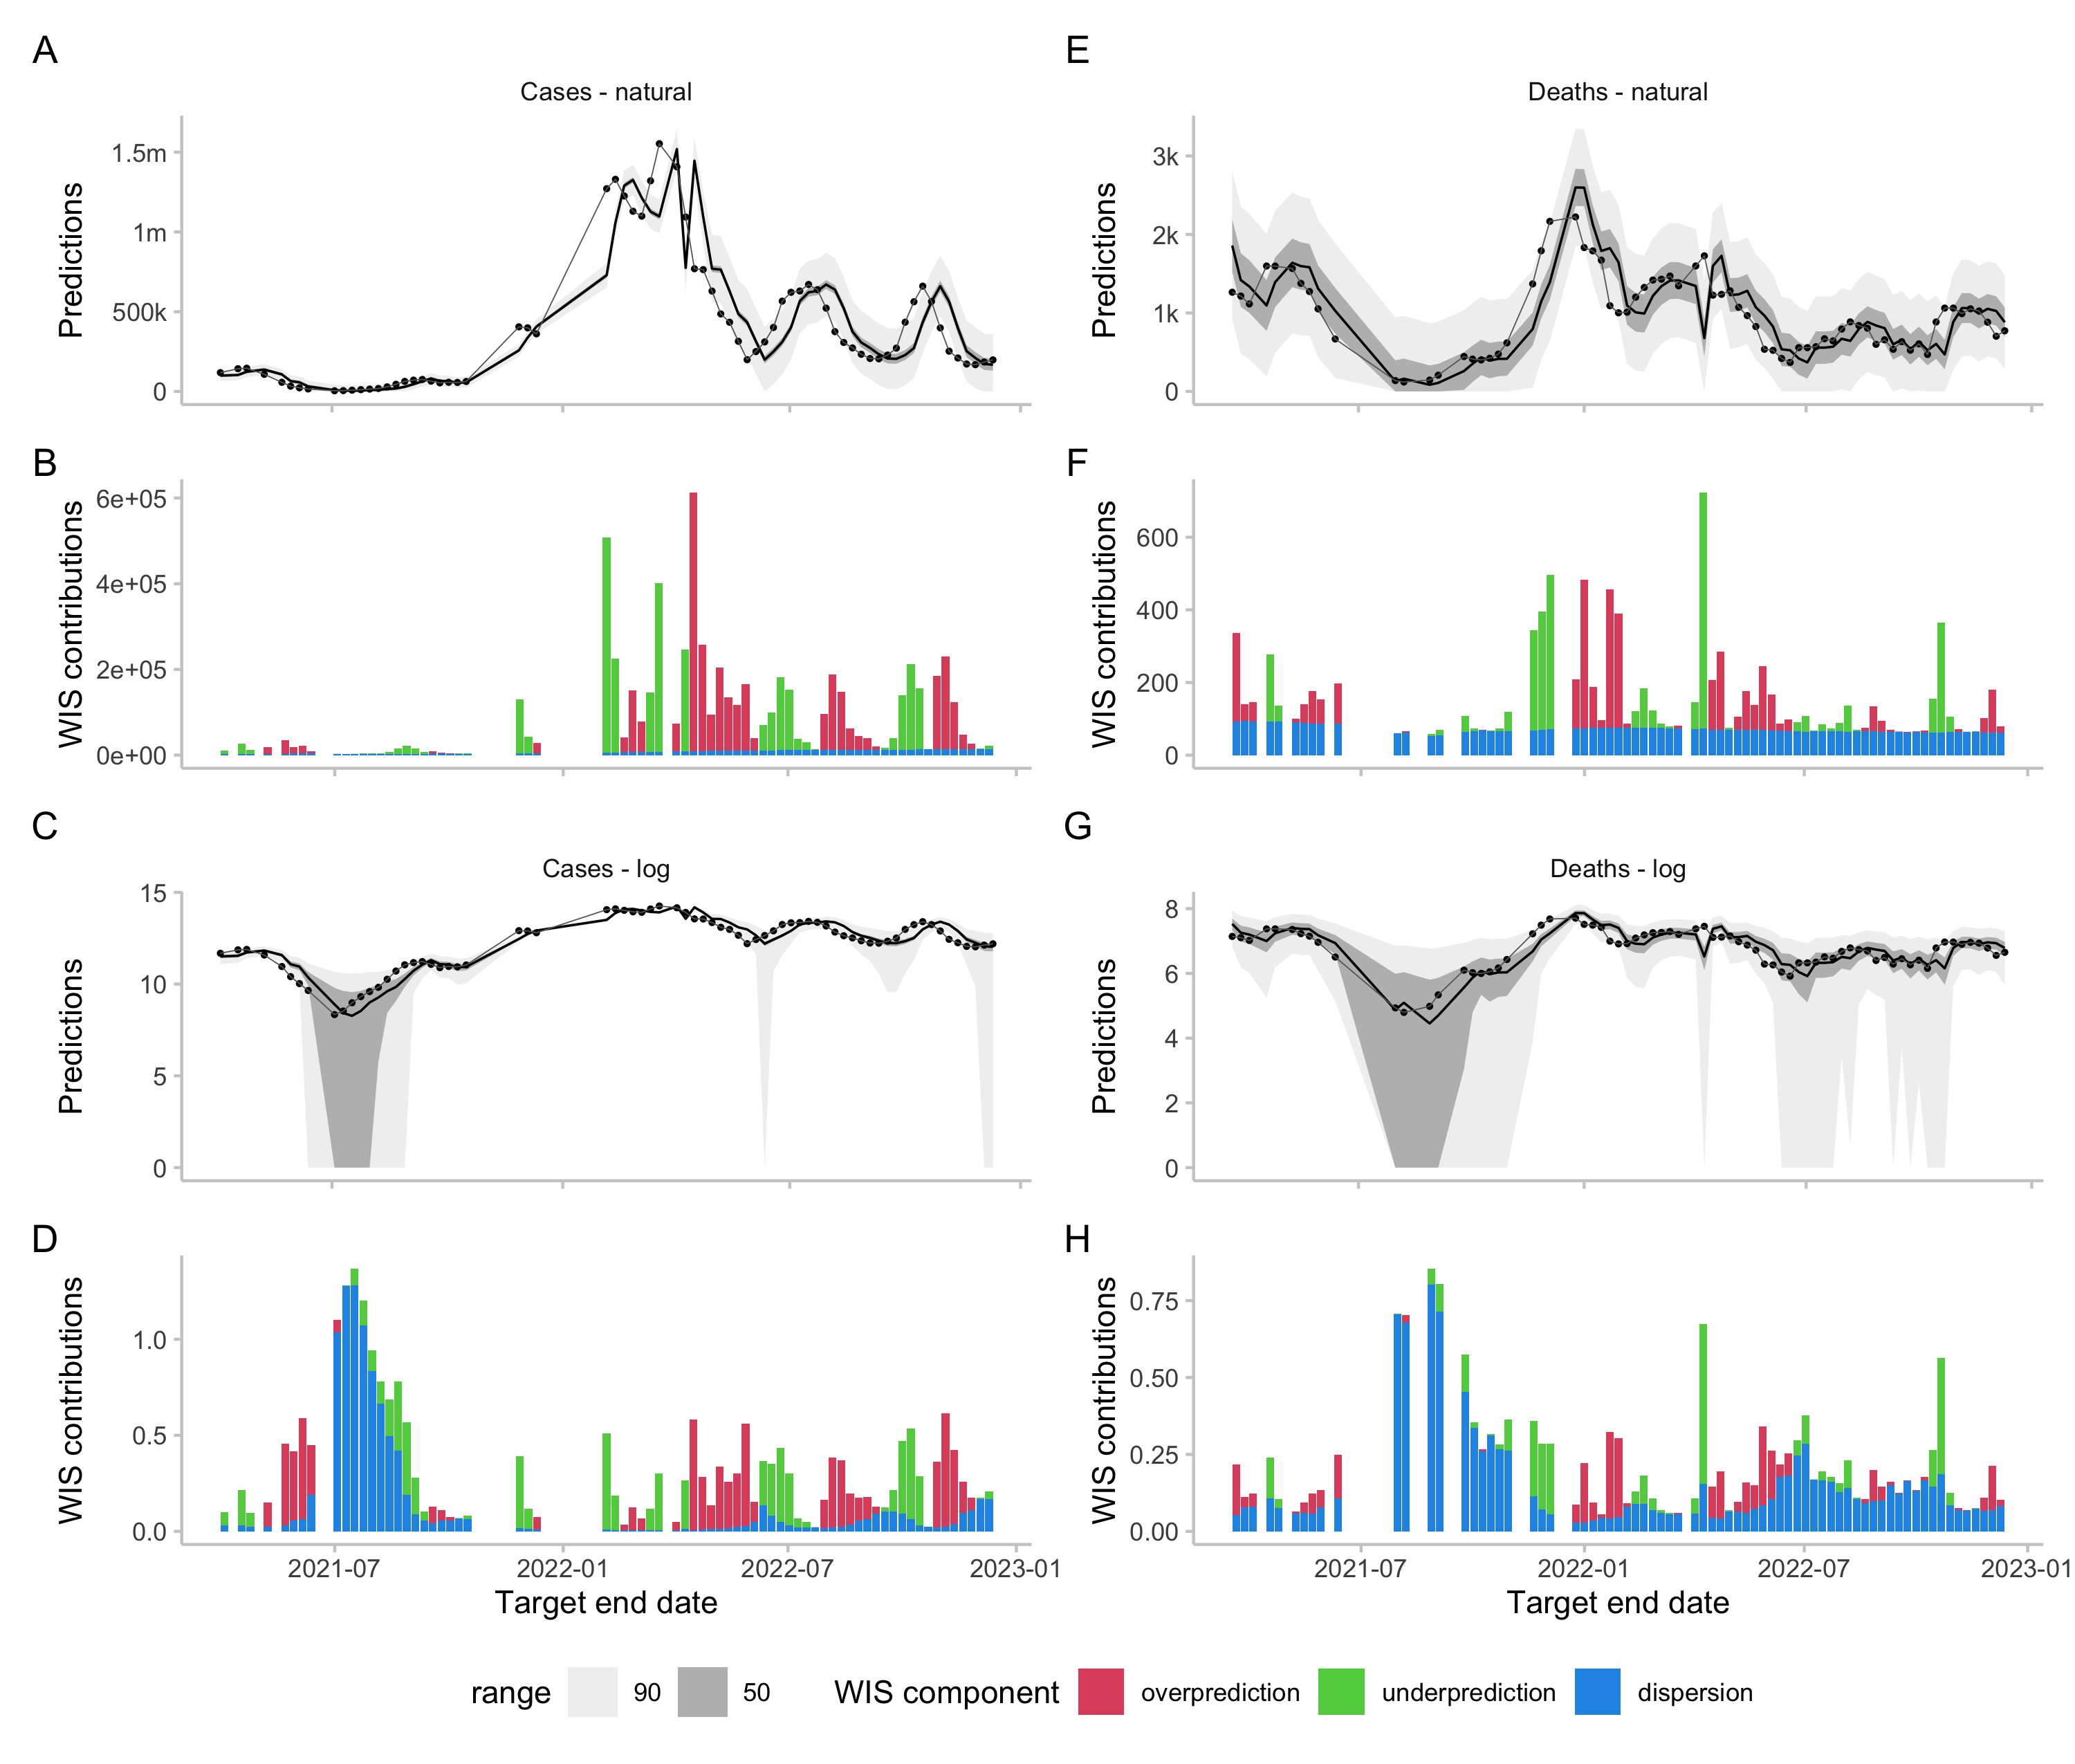
\includegraphics[width=0.99\textwidth]{output/figures/HUB-model-comparison-baseline.png}
    \caption{
    Forecasts and scores for two-week-ahead predictions from the EuroCOVIDhub-ensemble made in Germany. A, E: 50\% and 90\% prediction intervals and observed values for cases and deaths on the natural scale. B, F: Corresponding scores. C, G: Forecasts and observations on the log scale. D, H: Corresponding scores. 
    }
    \label{fig:HUB-model-comparison-baseline}
\end{figure}

\begin{figure}[h!]
    \centering
    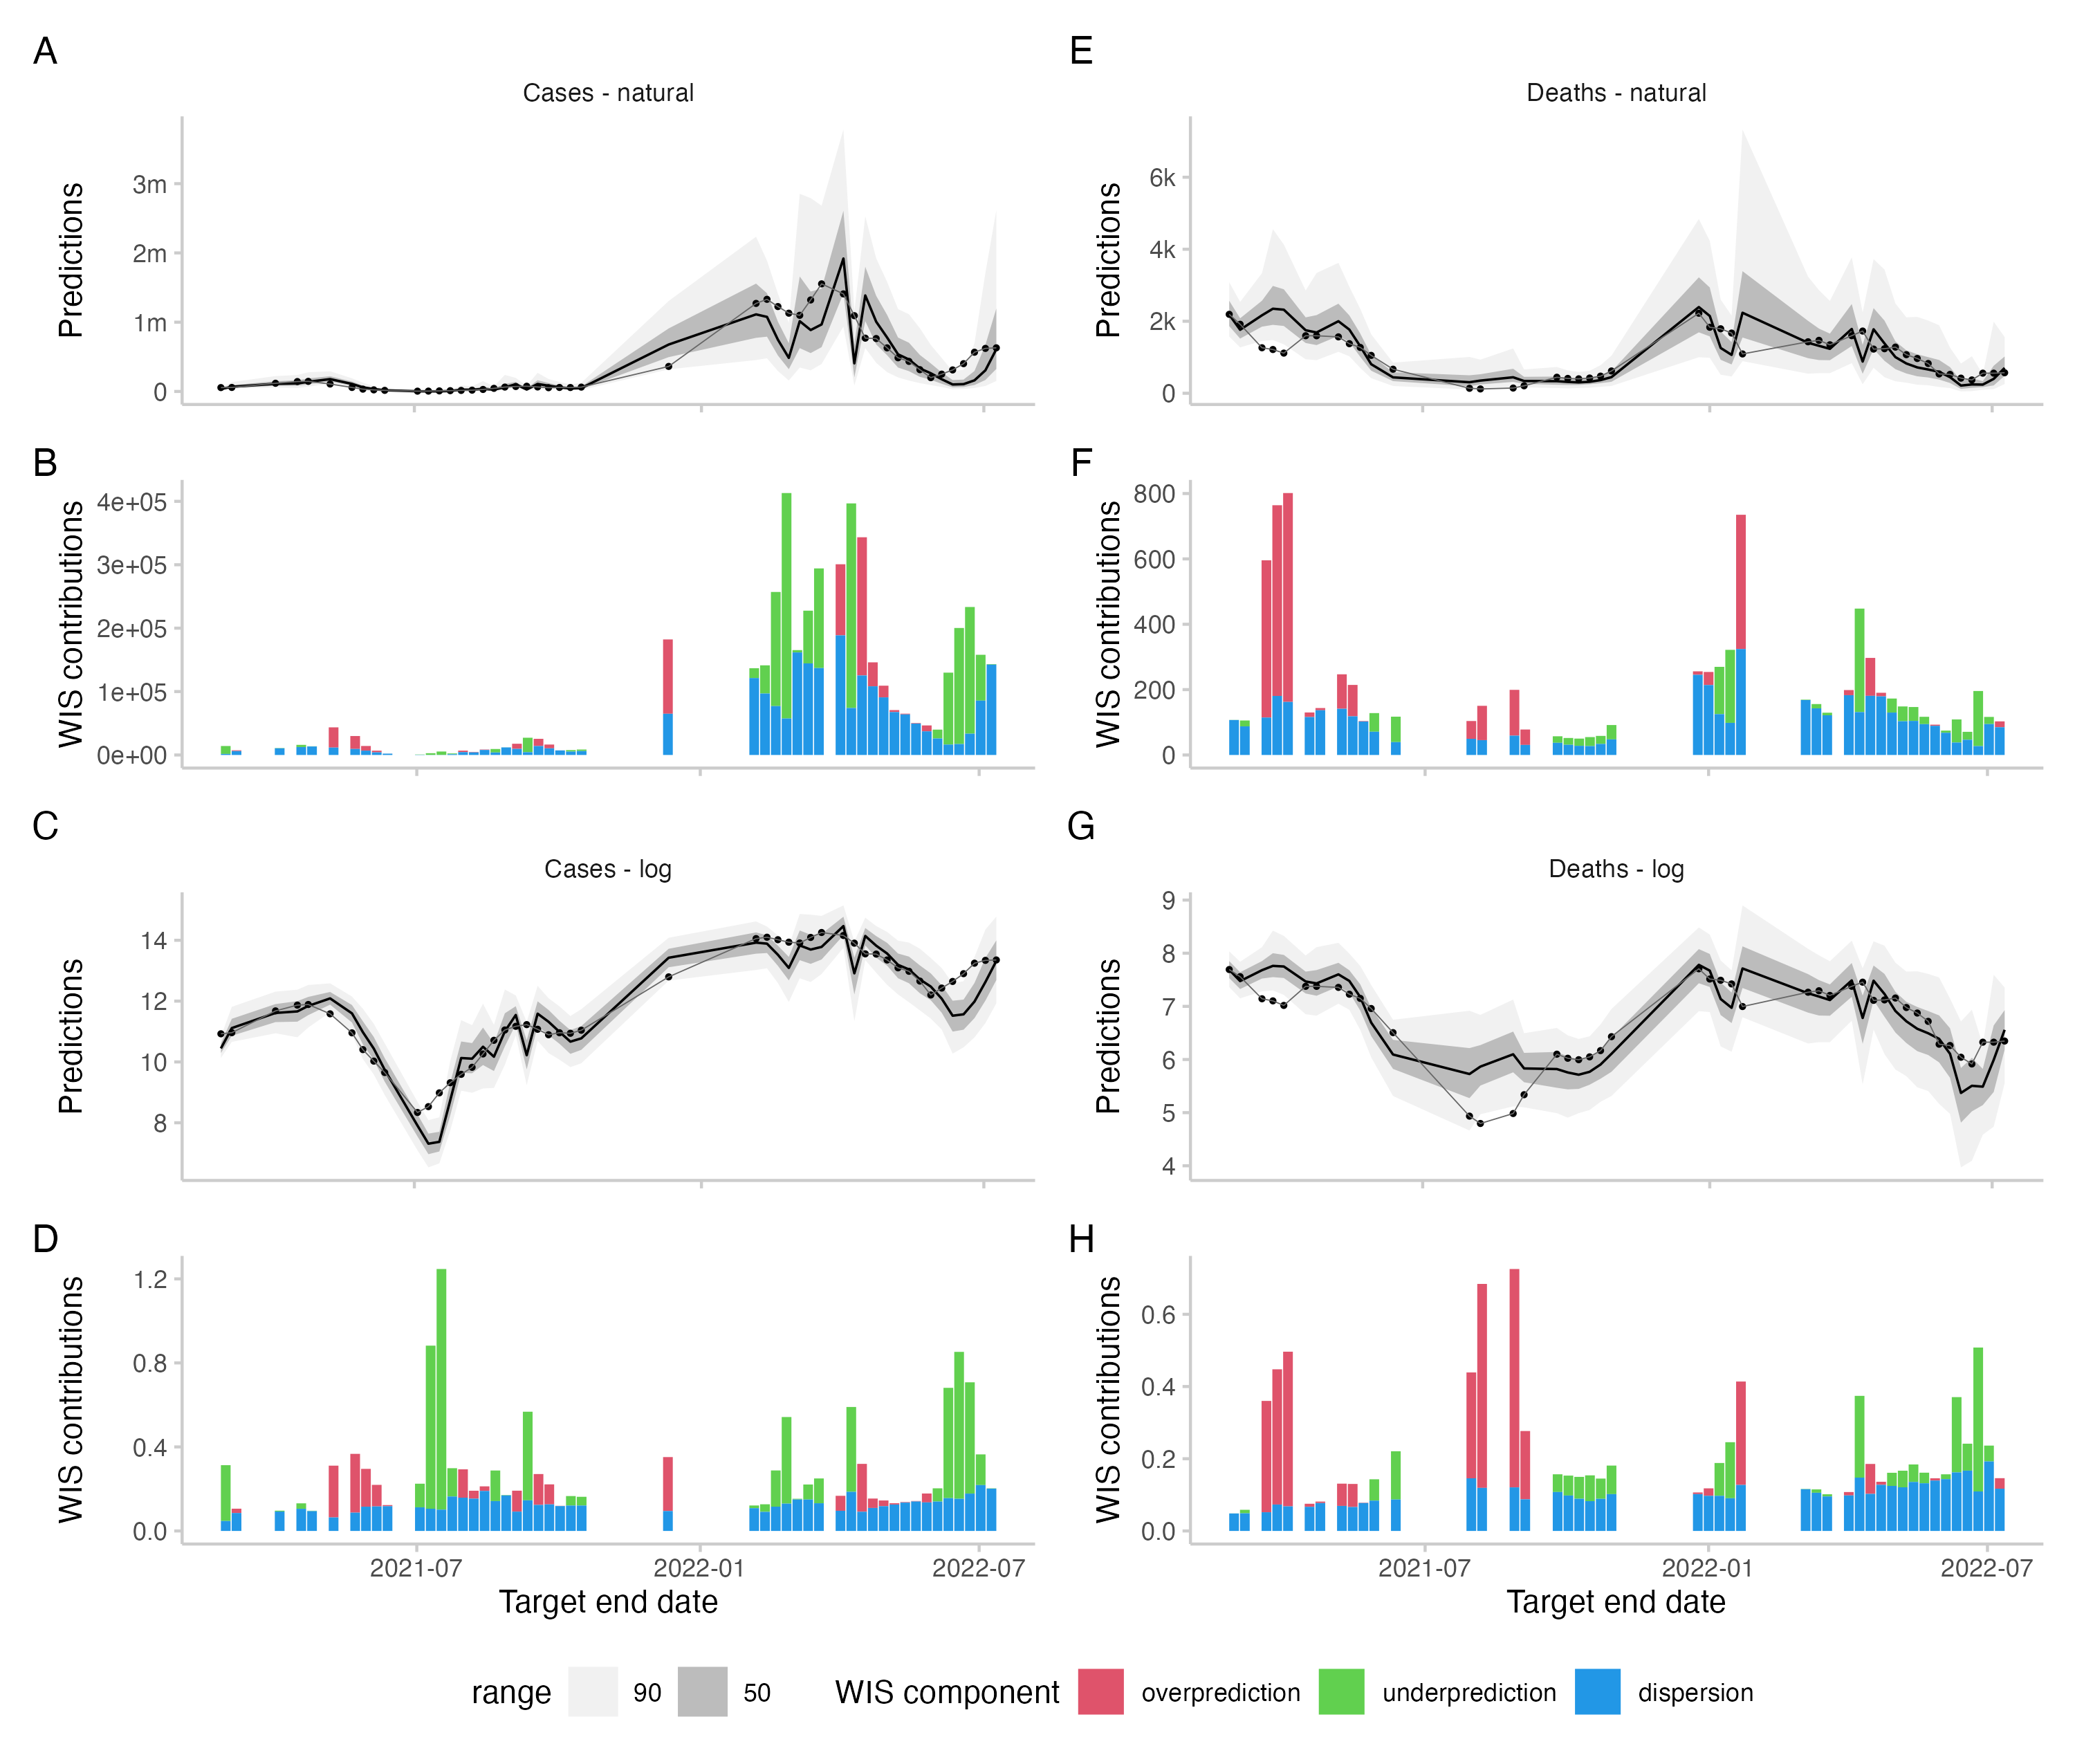
\includegraphics[width=0.99\textwidth]{output/figures/HUB-model-comparison-epinow.png}
    \caption{
    Forecasts and scores for two-week-ahead predictions from the EuroCOVIDhub-ensemble made in Germany. A, E: 50\% and 90\% prediction intervals and observed values for cases and deaths on the natural scale. B, F: Corresponding scores. C, G: Forecasts and observations on the log scale. D, H: Corresponding scores. 
    }
    \label{fig:HUB-model-comparison-epinow}
\end{figure}

\clearpage
\bibliography{log-or-not.bib}


\end{document}


%%%%%%%%%%%%%%%%%%%%%%%%%%%%%%%%%%%%%%%%%%%%%%%%%%%%%%%%%%%%%%%%%%%%%%%%%%%%
% Idea parking lot 
%%%%%%%%%%%%%%%%%%%%%%%%%%%%%%%%%%%%%%%%%%%%%%%%%%%%%%%%%%%%%%%%%%%%%%%%%%%%

% \section{Other ideas}
% \begin{itemize}
%     \item Compare different predictive distributions and the score as a function of an outcome.
%     \item ...
% \end{itemize}


%Score different things from the European / US Forecast Hub and plot the relationship between mean and variance. Plot log-scale scores for different things and see which of these influence average scores most \\
% What happens to the decomposition of the WIS if we log? 

%\begin{itemize}
%    \item Optional: Discussion of parallels to point forecasts and the point that you're still incentivised to report the median\\
%\end{itemize}




% NOT SO CONVINCED ANYMORE THAT THIS WORKS. MY INTUITION IS IF YOU WANT THE GROWTH RATE YOU SHOULD ACTUALLY SCORE THE GROWTH RATE AND DIVIDE BY THE LAST OBSERVED VALUE. 
% 
% WELL MAYBE IT WORKS AFTER ALL AND IT WOULD BE THE EQUIVALENT OF LOGGING FIRST AND THEN SUBTRACTING THE LAST OBSERVED VALUE WAIT A MINUTE THAT'S A DIFFERENT TRANSFORMATION AND ALSO THAT's SCORING THE LOG GROWTH RATE. 
% 
% BUT THEN AGAIN I'M STILL CONFUSED, BECAUSE ANY RELATIVE ERROR ON A QUANTITY Y\_t+1 IS AUTOMATICALLY AN ABSOLUTE ERROR ON THE GROWTH RATE IF WE KNOW Y\_t. AH BUT YOU DON'T KNOW WHAT THE ABSOLUTE ERROR ON THE GROWTH RATE IS (E.G. FOR Y\_t+1 of 10 IF YOU DON'T SPECIFICALLY LOOK AT THE LAST VALUE. BUT WE ARE ASSUMING THAT THIS IS WHAT THE MODEL DOES WHEN IT MAKES A FORECAST INTERNALLY




% The WIS can be thought of as an approximation of the CRPS for forecasts where the predictive distribution is represented through a set of quantiles. The CRPS, and by extension the WIS, represents a generalisation of the absolute error to continuous distributions, meaning that forecasters are evaluated on the absolute distance of their predictive distribution to the observed value (i.e. some form of absolute error). For simplicity, we will use absolute error and absolute distance between forecast and observation interchangeably, even though the former applies to point predictions and the latter is used for probabilistic forecasts. 


% 
% 
% 
% We argue that when dealing with epidemiological processes it makes sense to shift the evaluation towards multiplicative errors by either taking the logarithm of both the forecast and the observations or by dividing them by the last known observation before scoring. 

% What kinds of transformations can be considered meaningful depends on the context. We will illustrate the idea of transforming forecasts by focussing on the WIS as it is currently used in epidemiological settings such as the COVID-19 Forecast hubs. 
% In this paper we focus on the WIS due to its simplicity and widespread use by the COVID-19 Forecast Hubs, but arguments apply analogously to the CRPS. Another proper scoring rule commonly used is the log score [CITATION], which we will not discuss further in this paper. 


% \paragraph{Problems with the WIS and CRPS in an epidemiological setting}
% Their relation to the absolute error means that both the WIS and the CRPS usually scale with the prediction target. Forecasts of COVID-19 cases, for example typically have higher scores than forecasts of hospitalisations of death. Similarly, when looking at performance across different locations or over time, average scores will be dominated by locations and times with high incidences. Outliers also can have a disproportionate effect on aggregate scores. One can argue that this is meaningful and that we should care most about places and periods when incidence is high (maybe cite Bracher et al.). However, this may not always be true and is clearly not desirable when comparing performance of a model on different prediction targets: case numbers are not necessarily more important than hospitalisations, just because observed values tend be an order of magnitude higher. This makes forecasts often hard or impossible to compare. 


% not sure this plot is really meaningful
%\begin{figure}[h!]
%    \centering
%    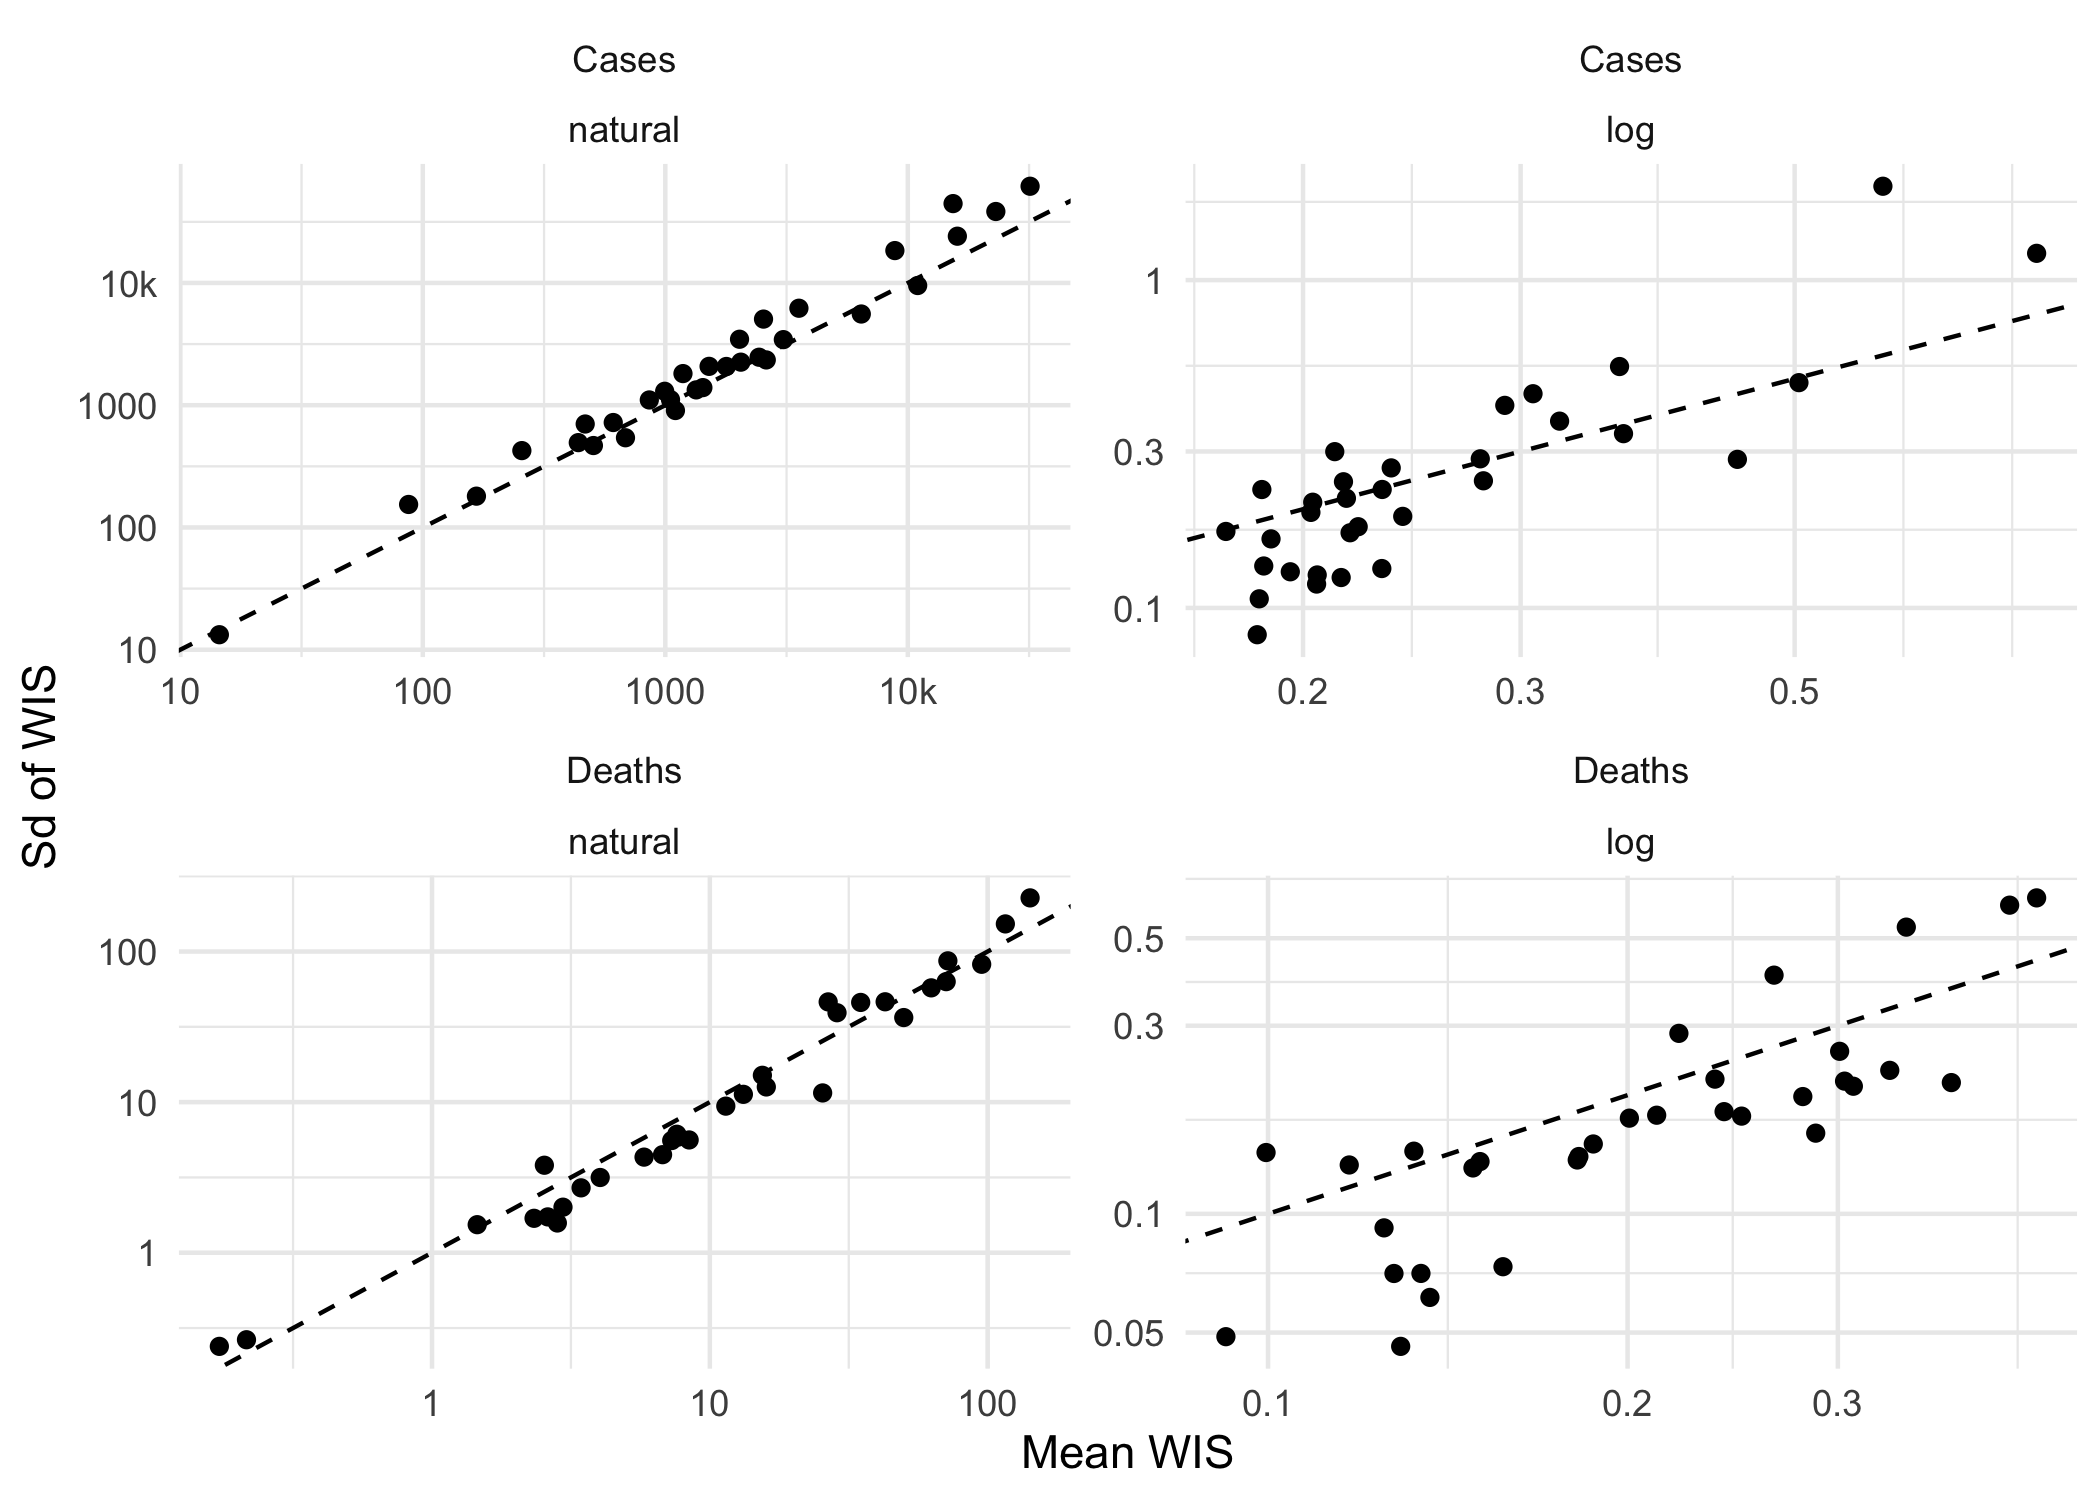
\includegraphics[width=0.99\textwidth]{output/figures/HUB-sd-vs-mean-scores.png}
%    \caption{CAPTION}
%    \label{fig:HUB-mean-sd-scores}
%\end{figure}

%\begin{itemize}
%    \item idea of scores on logged data: interpretation as a measure of relative improvement, just as when you log the absolute error
%\end{itemize}

%\paragraph{What's there in the literature}

%\paragraph{Current problems / questions about scoring an epidemiological setting}
%probably narrow down to the ones we really want to discuss%
%There are limitations with what we can do with scores on a natural scale and open questions whether we can do these things on a log-scale and also whether a log-scale might be inherently more appropriate
%\begin{itemize}
    %\item Can't really model score on a natural scale as errors are heavily skewed. Is there a way to model scores to get insight about different factors that systematically influence scores
 %   \item make a plot somewhere that shows the distribution of scores
  %  \item Maybe epidemiological forecasts are inherently better suited to be scored on an absolute scale due to the multiplicative nature of processes (related to over-prediction > under-prediction)? Does the log-scale imply we are scoring the growth rate? 
   % \item unclear what trade-offs of logging / not logging are
    %\item what score (log, not log) matches closest what our intuition (or policymakers) think is good? 
    %\item are we better at forecasting deaths than cases? --> relative measure would help
    %\item There exists confusion about what can be done to a score in general (e.g. people want to take the median, which they shouldn't) %maybe don't add as an extra point
%\end{itemize}


%\paragraph{Over- and under-prediction}
%If we want to keep this in, we could: 
%\begin{itemize}
%    \item Check whether there is actually a problem with over-prediction and under-prediction in the Hub. This could be the case because we are most interested in certain scenarios in which this might arise. 
%    \item Discuss this in light of Johannes' analysis of how the decomposition of WIS values differs if the data are skewed
%    \item compare this to the PIT-value-like relative bias scores we used for the German / Polish paper, which capture a relative tendency to over- or under-predict, rather than absolute penalties. 
%\end{itemize}


 % Pooled across all time points and locations, the mean WIS on the natural scale for cases (deaths) was 8855 (59.3) with an overall standard deviation of 51274 (156) (see Table \ref{tab:HUB-summary}). On the log scale, scores were much closer to each other (see Figure \ref{fig:HUB-average-scores}), with a mean WIS for cases (deaths) of 0.507 (0.362) with an overall standard deviation of 0.745 (0.407). 

% When evaluated on the natural scale, there is  strong relationship between the mean of the weighted interval score and the total number of observed cases (correlation: 0.913) or deaths (cor: 0.849) in a location (see Figure \ref{fig:HUB-mean-scores-total-loglog} and Figure \ref{fig:HUB-mean-scores-total} in the SI). The relationship is less pronounced for scores on the log scale (cor: -0.019 for cases, -0.395 for deaths) and negative, meaning that locations with fewer observed cases or deaths tend to receive higher scores. 


%Whether or not a log transformation is appropriate depends on whether one believes that differences in absolute values are meaningful. This may be the case for example when comparing forecasts across locations or time points, rather than different forecasts targets. \cite{bracherEvaluatingEpidemicForecasts2021} for example argue that in epidemiological settings it is a desirable property of the CRPS / WIS that it assigns large scores to forecasts where counts are high, as this naturally reflects the situations we should most care about and helps us identify the models that perform best in similar situations. If, on the other hand, we believe that good models should do consistently well and that situations with high incidences do not provide significantly more information about which models perform well or badly, then scoring on the log scale may be more appropriate. For example, it may be reasonable not to think that predictive performance in a country like Germany would have a hundred times more importance than performance in a country like Luxembourg when determining the best model for future decision making. Similarly, we may not necessarily believe that predictive performance during the January 2022 wave of COVID-19 should carry three times as much weight than predictive performance during the January 2021 wave, just because numbers where three times as high. 


% Divide by the latest known value = score forecast on the growth rate
% - WHAT KINDS OF DATA CAN I CONDITION ON? 
% - WOULD DIVIDING A FORECAST BY ITS RESOLUTION WORK? 
% - CAN I SCORE THE TRAJECTORY / WEEK-TO-WEEK GROWTH RATE BY DIVIDING the 4 week ahead forecast by the three week ahead forecast? 